% ========================================= TEMPLATE INFO ========================================
%
% Author:       P4ntomime
% Version:      1.0.0
% Last updated: 2024-02-18
% Brief:        A LaTeX template for summaries. See README.md for more information.
% 
% ================================================================================================
\documentclass[8pt, a4paper, twoside]{extarticle}
% Font size:    8pt
% Paper size:   A4
% style:        twoside (needed, so odd and even pages have different margins)
% orientation:  portrait. (use 'landscape' for landscape orientation)


% ========================================= DOCUMENT INFO =========================================
\def\title{Embedded Software Engineering 1}             % title
\def\shorttitle{EmbSW1}                                 % short title (displayed as PDF title)
\def\dozent{Prof. Reto Bonderer}                        % lecturer
\def\semester{HS 2024}                                  % semester
\def\author{Laurin Heitzer, Simone Stitz}               % author(s)
\def\repo{https://github.com/P4ntomime/EmbSW1}          % repository link
\def\version{1.0.\today}                                % version
\def\pagelimit{100}                                     % page limit -> causes pages after limit to be red
\def\titleoption{compact}                               % options: ultra compact, compact, normal
\def\enableToC{true}

% ================================= PACKAGES, SETUP AND COMMANDS ==================================
\input{preamble.tex}


% =========================================== DOCUMENT ============================================
\begin{document}
    \begin{layout}
        % Echtzeit- (real-time)Systeme, Multitasking, Scheduling, Rate Monotonic Scheduling
        \section{Embedded Systems -- Allgemein}
\subsection{Definition}

Ein Embedded System...

\begin{itemize}
    \item ist ein System, das einen Computer beinhaltet, selbst aber kein Computer ist
    \item besteht üblicherweise aus Hardware (Mechanik, Elektronik) und Software
    \item ist sehr häufig ein Control System (Steuerung, Regelung)
\end{itemize}

\vspace{0.2cm}

Ein Embedded System beinhaltet typischerweise folgende Komponenten:

\begin{minipage}[t]{0.15\columnwidth}
    \begin{itemize}
        \item Sensoren
        \item Aktoren
    \end{itemize}
\end{minipage}
\hfill
\begin{minipage}[t]{0.3\columnwidth}
    \begin{itemize}
        \item Mikrocomputer
        \item Software (Firmware)
    \end{itemize}
\end{minipage}
\hfill
\begin{minipage}[t]{0.45\columnwidth}
    \begin{itemize}
        \item Hardware (Mechanik, Elektronik)
    \end{itemize}
\end{minipage}


\subsubsection{Charakterisierung von Embedded Systems}

Embedded Systems können \textbf{(müssen aber nicht)} folgende Eigenschaften haben:

\begin{outline}
    \1 \textbf{reactive systems:}  Reaktive Systeme interagieren mit ihrer Umgebung
    \1 \textbf{real-time systems:} Echtzeitsysteme haben nebst funktionale Anforderungen auch definierbaren zeilichen Anforderungen zu genügen
    \1 \textbf{dependable systems:} Verlässliche Systeme sind Systeme, welche (sehr) hohe Zuverlässigkeitsanforderungen erfüllen müssen
    \1 \textbf{Weitere (häufige) Anforderungen:} 
        \2 kleiner Energieverbrauch
        \2 kleine physikalische Abmessungen
        \2 Lärm, Vibration, etc.
\end{outline}


\subsubsection{Typischer Aufbau}

\textbf{Ein gutes Design beinhaltet unterschiedliche Abstraktionsschichten \textrightarrow\ Layer} \\
\textrightarrow\ Siehe Abschnitt \ref{Hardware Abstraction Layer (HAL)}

\begin{center}
    \includegraphics[width=0.8\columnwidth]{images/embedded_system_aufbau_schichten.pdf}
\end{center}


\subsection{Beispiele}

\vspace{-0.2cm}

\begin{minipage}[t]{0.48\columnwidth}
    \raggedright
    \subsubsection*{Fahrrad-Computer}

    \begin{outline}
        \1 GPS-Navigation
        \1 Geschwindigkeits- und Trittfrequenzmessung
        \1 Pulsmesser
        \1 Drahtlosübertragung (ANT+)
        \1 Interface zu elektronischer Gangschaltung
        \1 Barometer, Thermometer
        \1 Trainingsassistent
        \1 Display
    \end{outline}

    \subsubsection*{Weitere Beispiele}

    \begin{itemize}
        \item Smartphone
        \item Mobile Base Station
        \item CNC-Bearbeitungszentdrum
        % \item Schubumkehr bei Flugzeugen
        % \item Lungenzustandsdetektion mit Elektro-Impedanztomographie (EIT)
        \item Hörgerät
    \end{itemize}
\end{minipage}
\hfill
\begin{minipage}[t]{0.48\columnwidth}
    \raggedright
    \subsubsection*{Auto}

    \begin{outline}
        \1 Sicherheitsrelevante Aufgaben
            \2 ABS, ASR
            \2 Motorenregelung
            \2 Drive-by-wire
            \2 Autonom fahrende Autos
        \1 Unterhaltung / Komfort
            \2 Radio / CD / etc.
            \2 Navigation
            \2 Klima
        \1 Mehrere Netzwerke
            \2 CAN, LIN, Ethernet
        \1 Echtzeitteile und andere
        \1 Von einfachsten $\micro$Cs bis DSPs und GPUs 
    \end{outline}

    \textrightarrow\ Auto ist ein riesiges Embedded System
\end{minipage}


\subsection{Deeply Embedded System}

\begin{itemize}
    \item 'Einfaches' Embedded System, mit \textbf{minimaler Benutzerschnittstelle}, üblicherweise mit \textbf{keinerlei GUI}
        und \textbf{ohne Betriebssystem}
    \item Beschränkt auf \textbf{eine} Aufgabe (z.B. Regelung eines physikalischen Prozesses)
    \item Muss oft zeitliche Bedingungen erfüllen \textrightarrow\ Echtzeitsystem
\end{itemize}


\subsubsection{Beispiele -- Deeply Embedded System}

\begin{minipage}[t]{0.3\columnwidth}
    \begin{itemize}
        \item Hörgerät
        \item Motorenregelung
    \end{itemize}
\end{minipage}
\hfill
\begin{minipage}[t]{0.3\columnwidth}
    \begin{itemize}
        \item ABS-Controller
        \item 'Sensor' im IoT
    \end{itemize}
\end{minipage}
\hfill
\begin{minipage}[t]{0.3\columnwidth}
    \begin{itemize}
        \item etc...
    \end{itemize}
\end{minipage}


\subsection{Betriebssysteme bei Embedded Systems}

\begin{outline}
    \1 Es kommen Betriebssysteme wie (Embedded) Linux oder Android zum Einsatz \\
        \textrightarrow\ \textbf{Achtung: Linux und Android sind nicht echtzeitfähig!}
    \1 Wenn Echtzeit verlangt wird: real-time operating systems (RTOS)
        \2 Beispiele: Zephyr, Free RTOS (Amazon), TI-RTOS (Texas Instuments), etc. \\
            \textrightarrow\ RTOS siehe Abschnitt \ref{Real-Time Operating Systems (RTOS)}
\end{outline}


\subsection{Bare Metal Embedded System}

\begin{itemize}
    \item Es kommt \textbf{keinerlei Betriebssystem} zum Einsatz
    \item Bare Metal Embedded Systems sind recht \textbf{häufig}, insbesondere bei \textbf{Deeply Embedded Systems}
    \item Bare Metal Embedded Systems stellen besondere Ansprüche an Programmierung
\end{itemize}


\subsection{Zuverlässigkeit}

\begin{minipage}[c]{0.45\columnwidth}
    \pgfplotsset{samples=100}   % sample points to make graph smooth

\begin{center}
    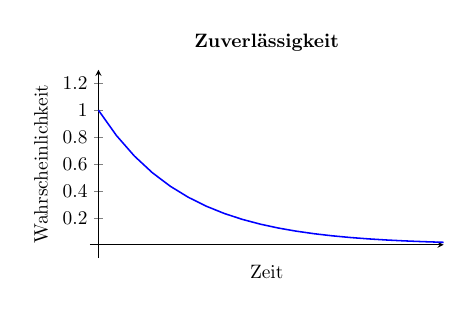
\begin{tikzpicture}
        [
            scale = 0.7,
            >=latex
        ]
        \begin{axis}
            [
                title=\textbf{Zuverlässigkeit},
                width=8cm,
                height=5cm,
                xmin=-0.2, xmax=8, ymin=-0.1, ymax=1.3, axis lines=middle,
                x label style={at={(axis description cs:0.5,0)},anchor=north},
                y label style={at={(axis description cs:-0.1,0.5)},rotate=90,anchor=south},
                xlabel=Zeit,
                ylabel=Wahrscheinlichkeit,
                xtick=\empty,
                ytick={0, 0.2, 0.4, 0.6, 0.8, 1, 1.2}
                %grid
            ]
        
            % plot
            \addplot[color=blue, thick, domain=-0:10]{exp(-0.5*x)};
        \end{axis}
        
    \end{tikzpicture}
\end{center}
\end{minipage}
\hfill
\begin{minipage}[c]{0.5\columnwidth}
    \raggedright

    \begin{itemize}
        \item Je länger das System läuft, desto weniger zuverlässig ist es
        \item Die Wahrscheinlichkeit für einen Ausfall steigt stetig
    \end{itemize}
    
    \vspace{0.2cm}

    \textbf{Achtung:} Hier ist nur die Alterung der Hardware berücksichtigt
\end{minipage}


\subsection{Verfügbarkeit}

Die Verfügbarkeit A (availability) ist der Anteil der Betriebsdauer innerhalb dessen das System seine Funktion erfüllt.
$$ \text{Verfügbarkeit} = \frac{\text{Gesamtzeit} - \text{Ausfallzeit}}{\text{Gesamtzeit}} $$


% \subsection{Abstraktionsschichten}

% \begin{itemize}
%     \item Bei $\micro$C-Programmierung (Firmware) müssen oft Bitmuster in Register geschrieben werden
%     \item Solche Register-Zugriffe dürfen \textbf{nicht} 'willkürlich' überall im Code erfolgen \\
%         \textrightarrow\ schlecht lesbar, schlecht portiertbar, fehleranfällig
%     \item \textbf{Damit Code lesbarer und besser auf andere Platform portierbar wird, beinhaltet jeder professionelle Code einen
%         Hardware Abstraction Layer (HAL)}
%     \item HAL führt \textbf{nicht} zum Verlust bei Laufzeit, wenn korrekt implementiert
% \end{itemize}


% \subsubsection{Hardware-abstraction-layer (HAL)}

% \begin{itemize}
%     \item Trennt HW-Implementierung von SW-Logik
%     \item Gleiche SW kann auf verschiedene HW verwendet werden \textrightarrow\ Portabilität
%     \item HW-Komponenten können einfach ausgetauscht werden \textrightarrow\ Flexibilität
% \end{itemize}


        % Modellierung von Embedded (real-time) Systems (Model Driven Development, MDD)
        \section{Real-Time System (Echtzeitsystem)}



        \section{Modellierung eines Embedded Systems}

\subsection{V-Modell für Software-Entwicklungszyklus}

\begin{center}
    \includegraphics[width=0.8\columnwidth]{images/V_modell.png}
\end{center}

\textrightarrow\ Nur Anforderungen (requirements) definieren, welche man auch testen kann!


\subsection{Model Driven Development (MDD)}

\begin{outline}
    \1 Bei \textbf{modellbasierter Entwicklung} kommen in \textbf{allen Entwicklungsphasen} durchgängig Modelle zum zur Anwendung
    \1 MDD geht davon aus, dass aus formalen Modellen lauffähige Software erzeugt wird \\
        \textrightarrow\ Codegeneratoren
    \1 Modelle werden traditionell als Werkzeug der Dokumentation angesehen
        \2 Unter Umständen wird zweimal dasslbe beschrieben (Code und Diagramm) \\
            \textbf{\textrightarrow\ unbedingt zu vermeiden!}
\end{outline}


\subsection{Vorgehen bei der Modellierung}

\begin{minipage}[c]{0.6\columnwidth}
    \begingroup
    \renewcommand{\outlinei}{enumerate}
    \renewcommand{\outlineii}{itemize}

    \begin{outline}
        \1  \cgn{Systemgrenze definieren}
            \2 Kontextdiagramm: Use-Case-Diagramm
            \2 Kontextdiagramm: Sequenzdiagramm
        \1 \cgn{Systemprozess finden}
            \2 Kontextdiagramm: Use-Case-Diagramm
            \2 Kontextdiagramm: Sequenzdiagramm
        \1 \cgn{Verteilungen festlegen}
            \2 Verteilungsdiagramm (deployment diagram)
        \1 \cbl{Systemprozesse detaillieren}
            \2 Umgangssprachlicher Text
            \2 Sequenzdiagramm
            \2 Aktivitätsdigramm
            \2 Statecharts
            \2 Code (C, C++, ...)
    \end{outline}
    \endgroup
\end{minipage}
\hfill
\begin{minipage}[c]{0.38\columnwidth}
    \raggedright
    \cgn{Stukturmodellierung (Statische Aspekte)}
    
    \vspace{0.2cm}

    \cbl{Modellierung der dynamischen Aspekte}
\end{minipage}


\subsection{Systemgrenze definieren \& Systemprozesse finden}

\subsubsection{Systemgrenze definieren}

\textbf{Die Festlegung der Systemgrenze ist das Wichtigste und Allererste bei sämtlichen Systemen!}

Man sollte sich die folgenden Fragen stellen und diese beantworten:

\vspace{0.1cm}

\begin{outline}
    \1 Was macht das System, d.h. was liegt innerhalb der Systemgrenze?
        \2 Was macht das System  \textbf{nicht}?
    \1 Mit welchen Teilen ausserhalb des Systems kommuniziert das System?
    \1 Welches sind die Schnittstellen zu den Nachbarsystemen (Umsystemen, periheral system)?
\end{outline}


\subsubsection{Systemprozesse finden (Use-Cases)}

Da man sich noch immer in der \textbf{Analyse} befindet, sollen nur die \textbf{Anforderungen} definiert werden. Die Umsetzung ist Teil
des Designs! \\
Um die Use-Cases zu identifizieren, sollte folgendes beachtet werden:

\vspace{0.1cm}

\begin{outline}
    \1 Aussenbetrachtung des Systems (\textbf{oberflächlich!})
        \2 Nicht komplizierter als nötig
    \1 System als Blackbox betrachten 
        \2 \textbf{Was} soll System können; (nicht: wie soll das System etwas machen)
    \1 RTE-Systeme bestehen häufig aus nur einem einzigen Systemprozess 
        \2 speziell wenn System 'nur' ein Regler ist
\end{outline}


\subsubsection{Kontextdiagramm: Use-Case Diagramm}

\begin{minipage}[t]{0.4\columnwidth}
    \myul{\textbf{Tempomat: zu detailliert}}

    \vspace{0.1cm}

    \includegraphics[width=\columnwidth]{images/use-case-diagramm_schlecht.png}
\end{minipage}
\hfill
\begin{minipage}[t]{0.48\columnwidth}
    \myul{\textbf{Tempomat: verbesserte Version}}

    \vspace{0.1cm}

    \includegraphics[width=\columnwidth]{images/use-case-diagramm_besser.png}
\end{minipage}


\subsubsection{Kontextdiagramm: Sequenzdiagramm}

\begin{itemize}
    \item Speziell bei Systemen, deren Grenzen durch \textbf{Nachrichtenflüsse} charakterisiert werden können
    \item Details zu Sequenzdiagrammen siehe Abschnitt \ref{Sequenzdiagramm}
\end{itemize}


\subsection{Verteilungen festlegen}

\begin{itemize}
    \item Bei Embedded Systems werden häufg \textbf{mehrere Rechnersysteme} verwendet, um die verschiedenen Aufgaben zu erledigen
    \item Rechner sind örtlich verteilt und mittels Kommunikationskanal verbunden \\
        \textbf{\textrightarrow\ Verteilte Systeme (distributed systems)}
\end{itemize}

\vspace{0.2cm}

\begin{minipage}[t]{0.5\columnwidth}
    \raggedright

    \subsubsection{Verteilungsdiagramm}
    
    \begin{description}
        \item[Knoten:] Darstellung der örtlichen Verteilung der Systeme \\
            Knoten können auch hierarchisch aufgebaut sein
        \item[Linien:] Physikalische Verbindungen der Knoten (Netzwerke, Kabel, Wireless, etc.)
    \end{description}
\end{minipage}
\hfill
\begin{minipage}[t]{0.46\columnwidth}
    \example{Tempomat}
    
    \includegraphics[width=\columnwidth]{images/verteilungsdiagramm_tempomat.png}
\end{minipage}


\subsection{Systemprozesse detaillieren}

\begin{outline}
    \1 Die gefundenen Systemprozesse (Use-Cases) müssen genauer spezifiziert werden
        \2 \textbf{Nicht detaillierter spezifizieren als sinnvoll / gefordert!}
        \2 Jede weitere Spezifizierung soll einen 'added value' liefern
    \1 Verschiedene Detaillierungsstufen für verschiedene Zielgruppen
        \2 Auftraggeber: Überblick (z.B. in Form von Umgangssprachlichem Text)
        \2 Systementwickler: 'Normale Sicht' enthält mehr Details
\end{outline}


\subsubsection{Sequenzdiagramm}
\label{Sequenzdiagramm}

\begin{minipage}[t]{0.48\columnwidth}
    \begin{outline}
        \1 Gute Darstellung für \textbf{Austausch von Meldungen} zwischen Objekten innerhalb einer \textbf{beschränkten Zeitdauer}
            \2 Nachrichtenflüsse
            \2 Kommunikationsprotokolle
    \end{outline}
\end{minipage}
\hfill
\begin{minipage}[t]{0.48\columnwidth}
    \begin{outline}
        \1 Ideal für...
            \2 kurze Zeitdauer
            \2 wenige Objekte
            \2 wenige Verschachtelungen
            \2 wenige Verzweigungen
    \end{outline}
\end{minipage}


\begin{center}
    \includegraphics[width=0.9\columnwidth]{images/sequenzdiagramm_elemente_1.png}

    \vspace{0.3cm}

    \includegraphics[width=0.9\columnwidth]{images/sequenzdiagramm_elemente_2.png}
\end{center}


\begin{minipage}[c]{0.45\columnwidth}
    \includegraphics[width=\columnwidth]{images/sequenzdiagramm_pfeile.png}
\end{minipage}
\hfill
\begin{minipage}[c]{0.52\columnwidth}
    \begin{itemize}
        \item Beim Zeichnen von Hand unbedingt die \textbf{Pfeilkonventionen} beachten!
        \item Diagramme generell nicht 'überladen'
    \end{itemize}
\end{minipage}

\columnbreak


\subsubsection{Kommunikationsdiagramm (Kollaborationsdiagramm)}

\begin{outline}
    \1 Kommunikationsdiagramm zeigt \textbf{dieselbe Information} wie Sequenzdiagramm
    \1 \textbf{Schwerpunkt: Informationsfluss} zwischen den Objekten \\
    \textrightarrow\ Beim Sequenzdiagramm liegt der Schwerpunkt auf dem zeitlichen Ablauf
\end{outline}

\begin{center}
    \includegraphics[width=0.7\columnwidth]{images/kommunikationsdiagramm.png}
\end{center}


\subsubsection{Aktivitätsdigramm}

\begin{minipage}[t]{0.48\columnwidth}
    \begin{outline}
        \1 Gut geeignet für ...
            \2 \textbf{workflow modelling}
            \2 Sequenzielle Abläufe
            \2 Prozess- und Steuerfluss
            \2 Gleichzeitige Prozesse (fork, join)
    \end{outline}
\end{minipage}
\hfill
\begin{minipage}[t]{0.48\columnwidth}
    \begin{outline}
        \1 Weniger geeignet für ...
            \2 komplexe logische Bedingungen
    \end{outline}
\end{minipage}


\begin{center}
    \includegraphics[width=0.8\columnwidth]{images/aktivitaetsdiagramm_elemente.png}

    \vspace{0.3cm}

    \includegraphics[width=0.8\columnwidth]{images/aktivitaetsdiagramm_parallelitaet.png}
\end{center}


        % Hardware/Software Codesign
        \section{Hardware-Software-Codesign}

\subsection{Ziele}

\begin{itemize}
    \item Entwurf (Design) \textbf{so lange wie sinnvoll} (nicht so lange wie möglich) \textbf{lösungsneutral}
    \item \textbf{Systemdesign fördern}, statt separate Designs für Mechanik, Elektronik, Firmware, Software, etc., die sich
        unter Umständen auch widersprechen können
    \item Systemspezifikation erfolgt idealerweise mit Hilfe einer \textbf{eindeutigen Spezifikationssprache}, nicht in
        Prosa
    \item Die Spezifikation sollte simuliert (ausgeführt) werden können
    \item Implementationen können einfach geändert werden: HW \textlrarrow\ SW
    \item Zielplattformen: diskrete Elektronik, ASIC, \micro C, DSP, \textbf{FPGA}, Software
\end{itemize}


\subsection{Anforderungen für praktische Anwendungen}

\begin{outline}
    \1 Methoden / Tools sollten beim Systemdesign nicht zu fachlastig sein
        \2 Methoden sollten für Elektronik-, Firmware- und wenn möglich auch Mechanikentwickler anwendbar sein
    \1 Wenn möglich gute Toolunterstützung
    \1 (Automatische Synthese aus dem Modell)
\end{outline}


\subsection{Spezifikationssprachen}

\begin{minipage}[t]{0.48\columnwidth}
    \raggedright
    \begin{itemize}
    \item \textbf{Formale Sprachen sind eindeutig} \\
        (Prosa immer mehrdeutig)
    \item Spezifikation kann compiliert und ausgeführt werden \textrightarrow\ Simulationen
    \item Die ausführbare Spezifikation dient als \textbf{Golden Reference} für die künftigen Entwicklungsschritte
\end{itemize}
\end{minipage}
\hfill
\begin{minipage}[t]{0.48\columnwidth}
    \myul{\textbf{Beispiele für Spezifikationssprachen}}

    \vspace{0.1cm}

    \begin{itemize}
        \item SystemC (eine C++-Template Library)
        \item SysML
        \item SpecC
        \item SystemVerilog
        \item Esterel
        \item Matlab/Simulink
        \item Statecharts
    \end{itemize}
\end{minipage}


\subsection{Virtuelle Prototypen}

\begin{itemize}
    \item Die Simulation des Systems kann unterschiedlich stark detailliert werden
    \item \textbf{Die simulierten Systeme sind Virtuelle Prototypen}
    \item Während der Entwicklung können einzelne (virtuelle) Teile des Prototyps laufend durch physische Teile
        ersetzt werden
\end{itemize}


\subsection{X-in-the-loop}

\begin{outline}
    \1 \textbf{Model-in-the-Loop (MIL):} vollständig als Modell vorliegender virtuellen Prototyp
    \1 Je mehr der Prototyp durch konkretere Implementationen ersetzt wird, spricht man von
        \2 Software-in-the loop (SIL)
        \2 Processor-in-the loop (PIL)
        \2 Hardwarein-the loop (HIL)
\end{outline}

\vspace{0.2cm}

\textrightarrow\ Test outputs werden jeweils mit \textbf{Golden Reference} verglichen
\begin{center}
    \includegraphics[width=0.9\columnwidth]{images/x_in_loop_testing.png}
\end{center}


\subsection{Entwicklungsplattformen}

Als Entwicklungsplattformen eignen sich häufig \textbf{FPGA basierte Systeme.}

\begin{outline}
    \1 Hardware mit VHDL
    \1 Software/Firmware in C/C++
        \2 auf integriertem \micro C (z.B. Zynq von AMD/Xilinx) (Hard core)
        \2 auf Soft Core innerhalb FPGA (z.B. Nios II von Intel/Altera)
\end{outline}


        % Finite State Machines (Anwendung, Implementationen in C und C++)
        \section{Zustandsbasierte Systeme}

\subsection{Asynchrone vs. synchrone FSM}

\begin{minipage}[t]{0.48\columnwidth}
    \raggedright
    \begin{outline}
        \1 \textbf{Asynchron}
            \2 geänderte Inputsignale führen \textbf{direkt} zur Zustandsänderung
            \2 schneller, aber enorm anfällig auf Glitches
    \end{outline}
\end{minipage}
\hfill
\begin{minipage}[t]{0.48\columnwidth}
    \raggedright
    \begin{outline}
        \1 \textbf{Synchron}
            \2 Inputsignale werden nur zu diskreten Zeitpunkten betrachtet \\
                \textrightarrow\ getaktete Systeme
    \end{outline}
\end{minipage}

\vspace{0.2cm}
%TODO: check if this is finished
\begin{outline}
    \1 Softwareimplementationen sind eigentlich immer \textbf{synchron}, da Rechner getaktet sind
    \1 Rein softwareseitig besteht die Problematik der Asynchronizität nicht
\end{outline}


\subsection{Finite State Machines (FSM)}


\subsubsection{Mealy-Automat}

\subsubsection{Moore-Automat}
% Bondi: alles als Moore modellieren

\subsubsection{Medvedjev}
%hier nicht weiter behandelt...?
% Zustand = Output


\subsection{State-Event-Diagramm (Zustandsdiagramm)}

% Beschreibung


\example{State-Event-Diagramm -- Moore Automat}

% \begin{center}
%     \includegraphics[width=0.8\columnwidth]{images/state_event_example.png}
% \end{center}


        \section{Statecharts}

\subsection{Nachteile von State-Event-Diagrammen}


\subsection{Hierarchie im Statechart}



        \section{Realisierung flache FSM}

\subsection{Mögliche Realisierungen von flachen FSMs}

\begin{outline}
    \1 Steuerkonstrukt (typischerweise mit \textbf{switch-case})
        \2 prozedural oder objektorientiert
    \1 Definition und Abarbeitung einer \textbf{Tabelle}
        \2 prozedural oder objektorientiert
    \1 \textbf{State Pattern} (Gang of Four, GoF)
        \2 nur objektorientiert
    \1 Generisch mit Templates
        \2 nur mit einer Sprache, die Templates unterstützt (z.B. C++)
\end{outline}

\vspace{0.2cm}

\textrightarrow\ Alle Varianten haben wie immer sowohl Vor- als auch Nachteile \\
\textrightarrow\ Bei allen Varianten sind auch Variationen vorhanden


\subsection{Realisieurng mit Steuerkonstrukt (prozedural in C)}

\subsubsection{State-Event-Diagram -- Up/Down-Counter}

\begin{center}
    \includegraphics[width=0.7\columnwidth]{images/fsm_up-down-counter_diagramm_C.png}
\end{center}


\subsubsection{Implementation der Prozeduralen Realisierung in C}

\begin{outline}
    \1 \textbf{Ereignisse (events)}
        \2 Schnittstelle nach aussen \textrightarrow\ ändern Zustand der FSM
        \2 In enum definiert (\textbf{public}) \textrightarrow\ header-file
        \2 Einzelne Events und enum Bezeichnung enthalten \textbf{Unitkürzel} (hier: \mylstbox{cnt_})
    \1 \textbf{Zustände (states)}
        \2 In enum definiert (\textbf{nicht} public) \textrightarrow\ sourcecode-file
    \1 \textbf{Aktueller Zustand} wird in einer \textbf{statischen Varianlen} gehalten
    \1 Die FSM wird in \textbf{zwei Funktionen} implementiert
        \2 Initialiserungs-Funktion (hier: \mylstbox{void cnt_ctrlInit(int initValue)})
        \2 Prozess-Funktion (hier: \mylstbox{void cnt_ctrlProcess(cnt_Event e)}) \\
            \textrightarrow\ Zustände prüfen, Zustandsübergänge veranlassen
    \1 Anstossen einer FSM
        \2 Initialisierung in \lstinline|main|-Funktion
        \2 Überprüfung, welches Event aufgetreten ist meist in \mylstbox{do-while}-Schleife
\end{outline}


\subsubsection{Implementation der Prozeduralen Realisierung in C}

\begin{outline}
    \1 Da aktueller Zustand eine statische Variable ist, kann es nur \textbf{eine einzige Instanz} der FSM geben
    \1 Bei mehreren Instanzen in C...
        \2 darf \mylstbox{currentState} nicht \mylstbox{static} sein und muss als Parameter mitgegenen werden,
            bzw. ein Pointer auf die jeweilige Variable
        \2 Zustands-enum muss in die Schnittstelle (header-file) oder es muss z.B. mit \mylstbox{void*} gearbeitet werden
    \1 In C ist \textbf{keine schöne Kapselung} der Attribute möglich (\mylstbox{currentState})
    \1 Funktion \mylstbox{cnt_ctrlProcess()} kann beliebig aufgerufen werden (periodischer Task, laufend, etc.)
    \1 Bei exponierten Funktionen / Definitionen muss in C ein Unitkürzel vorangestellt werden (hier: \mylstbox{cnt_})
\end{outline}


\example{UpD/Down-Counter (prozedural in C)}

% TODO: \para environment not showing...?
% TODO: add keywords an stuff to listings setup

\para{Schnittstelle FSM} 
\lstinputlisting{snippets/fsm_counterCtrl_C.h} 


\para{Implementation FSM} 
\lstinputlisting{snippets/fsm_counterCtrl_C.c}

\para{Anstossen der FSM} 
\lstinputlisting{snippets/fsm_main_counterTest.c}

\columnbreak


\subsection{Realisieurng mit Steuerkonstrukt (objektorientiert in C++)}

% \begin{center}
%     \includegraphics[width=0.7\columnwidth]{images/fsm_up-down-counter_diagramm_CPP.png}
% \end{center}


\subsection{Realisierung mit Tabelle}


\subsubsection{Performancesteigerung mit inline-Funktionen}


\subsubsection{Execution Engine}
        \section{Modularisierung}

Ziel der Modularisierung ist eine \textbf{Reduktion der Komplexität.}
$$ \sum_{i} \text{complexity(problem)}_i < \text{complexity} \Big( \sum_{i} \text{problem}_i \Big) $$

\vspace{-0.2cm}


\subsection{Grundprinzip Modularisierung}

\begin{outline}
    \1 \textbf{Problem in (einfachere) Unterprobleme aufteilen} und diese Unterprobleme jeweils \textbf{einzeln angehen}
    \1 Abstraktion 
\end{outline}


\subsubsection{Motivation für Modularisierung}

\begin{outline}
    \1 \textbf{Grosse Projekte -- 'richtige' Softwaresysteme}
        \2 Systematischer Designansatz und strukturierter Aufbau ermöglichen effiziente \textbf{Arbeit im Team}
        \2 Schnittstellen müssen klar definiert werden
    \1 \textbf{Informatin Hiding}
        \2 Für die Nutzung eines Moduls (Unit) muss es gnügen, \textbf{nur die Schnittstellen} zu kennen
\end{outline}


\subsubsection{Phasenunterteilung beim Entwurf}

\begin{outline}
    \1 \textbf{Grobentwurf, Architektur (architectural design)}
        \2 (Software-) System im Grossen
        \2 Schnittstellen zu anderen (Nicht-Software-) Systemen
        \2 Datenstruktur im Grossen
        \2 \textbf{Aufteilung in Subsysteme}
        \2 \textbf{Schnittstellen zwischen Subsystemen}
    \1 \textbf{Feinentwurf}
        \2 Innenleben und Datenstruktur im Kleinen
\end{outline}


\subsection{Bewertung einer Zerlegung}

\begin{outline}
    \1 \textbf{Kopplung (coupling)}
        \2 Mass für Komplexität der Schnittstelle
    \1 \textbf{Kohäsion (cohesion)}
        \2 Aussage, wie stark eine funktionale Einheit wirklich zusammengehört
        \2 Mass die die Stärke des inneren Zusammenhangs
\end{outline}

\vspace{0.1cm}

\textbf{ \textrightarrow\ Ziel ist eine schwache Kopplung mit starker Köhäsion!}


\subsection{Kopplung}

\vspace{-0.2cm}

\begin{tikzpicture}[baseline=(current bounding box.north), >=latex]
    \node[anchor=north west] (kopplung) {
        \begin{minipage}{0.8\columnwidth}
            \begin{outline}
                \1 \textbf{Keine direkte Kopplung}
                \1 \textbf{Datenkopplung}
                    \2 Kommunikation ausschliesslich über Parameter
                \1 \textbf{Datenbereichskopplung}
                    \2 Ein Modul hat Zugriff auf eine Datenstruktur eines anderen Moduls. Es werden allerdings nur einzelne
                        Komponenten wirklich benötigt.
                \1 \textbf{Steuerflusskopplung} (control flow)
                    \2 Ein Modul beeinflusst Steuerfluss eines anderen Moduls
                \1 \textbf{Globale Kopplung}
                    \2 Kommunikation über globale Variablen, jedes Modul hat Zugriff
                \1 \textbf{Inhaltskopplung (Todsünde!)}
                    \2 Aus einem Modul heraus werden lokale Daten eines anderen Moduls modifiziert, obwohl dieses Modul
                        gar nicht vom anderen Modul aufgerufen wird.
            \end{outline}
        \end{minipage}
    };

    % Vertical arrow
    \draw[->, thick] ([xshift=-1em]kopplung.south west) -- ([xshift=-1em]kopplung.north west)
        node[very near start, left, color=red, thick]   {\shortstack{ \textbf{stark} \\ \textbf{(schlecht)}} }
        node[very near end, left, color=green]          {\shortstack{ \textbf{schwach} \\ \textbf{(gut)}} };
\end{tikzpicture}


\subsection{Kohäsion}

\vspace{-0.2cm}

\begin{tikzpicture}[baseline=(current bounding box.north), >=latex]
    \node[anchor=north west] (cohesion) {
        \begin{minipage}{0.8\columnwidth}
            \begin{outline}
                \1 \textbf{funktional}
                    \2 Die Teile einer Einheit bilden zusammen eine Funktion, bzw. eine Funktionsgruppe
                \1 \textbf{sequentiell}
                    \2 Teilfunktionen einer Einheit werden nacheinander ausgeführt, wobei das Resultat einer
                        Funktion als Eingabe für die nächste verwendet wird
                \1 \textbf{kommunikativ}
                    \2 Die Teilfunktionen einer Einheit werden auf den gleichen Daten ausgeführt, Reihenfolge
                        spielt keine Rolle
                \1 \textbf{prozedural}
                    \2 Teilfunktionen werden nacheinander ausgeführt, verknüpft über Steuerfluss
                \1 \textbf{\cbl{zeitlich}}
                    \2 Die Teile einer Einheit sind alle zu einer bestimmten Zeit auszuführen
                    \2 Typischer Fall: alle Initialisierungsfunktionen werden zusammengefasst
                \1 \textbf{logisch}
                    \2 (nicht zusammengehörende) Teilfunktionen einer Einheit gehören zu einer Einheit
                \1 \textbf{zufällig}
                    \2 Die Teilfunktionen einer Einheit haben keinen sinnvollen Zusammenhang
            \end{outline}
        \end{minipage}
    };

    % Vertical arrow
    \draw[->, thick] ([xshift=-1em]cohesion.south west) -- ([xshift=-1em]cohesion.north west)
        node[very near start, left, color=red, thick]   {\shortstack{ \textbf{schwach} \\ \textbf{(schlecht)}} }
        node[very near end, left, color=green]          {\shortstack{ \textbf{stark} \\ \textbf{(gut)}} };
\end{tikzpicture}


\subsubsection{Ziele bezüglich Kohäsion}

\begin{outline}
    \1 Kohäsion soll maximiert werden \\
        \textbf{ \textrightarrow\ starke Kohäsion führt automatisch zu schwacher Kopplung!}
    \1 Den genauen Wert der Kohäsion zu ermitteln ist \textbf{kein} Ziel
\end{outline}

\vspace{0.1cm}

\textbf{ \textrightarrow\ Zusammengehörendes zusammennehmen!}


\subsection{Guidelines -- gute Modularisierung}

\begin{outline}
    \1 \textbf{Zusammengehörendes zusammennehmen}
        \2 Defines für spezigisches Modul in Header-File des Moduls
    \1 Passende / aussagekräftige Namen für Variablen
    \1 'Interne' (private) Funktionen in \mylstbox{.c}-file deklarieren und definieren
    \1 Schnittstellenbeschreibung in Header-Dateien
        \2 Falls möglich: Doxygen verwenden
    \1 Lokale Funktionen (z.B. in \mylstbox{main.c}) bei Funktionsdeklarationen kommentieren
    \1 Allenfalls 'globalen' Header für Typdefinitionen
        \2 besser: Typen aus \mylstbox{stdint.h} verwenden
    \1 \mylstbox{uint8_t} etc. verwenden, wenn gezielt ein 8 Bit register angesprochen wird (und nur dann!)
    \1 Keine \mylstbox{initialization.h} Dateien \textrightarrow\ zeitliche Kohäsion!
        \2 generell keine Dateien wie: \mylstbox{global.h}, \mylstbox{defines.h}, \mylstbox{util.h}, \mylstbox{project.h}
\end{outline}

\vspace{0.2cm}

\textbf{Hinweis:} Für die Zurechtfindung in einem bestehenden Projekt müssen generell immer zuerst die \textbf{Header-Files studiert werden!}


\example{Schlechte vs. gute Modularisierung}

\begin{minipage}[t]{0.48\columnwidth}
    \includegraphics[width=\columnwidth, align=t]{images/modulaisierung_bsp_schlecht.pdf}
\end{minipage}
\hfill
\begin{minipage}[t]{0.48\columnwidth}
    \includegraphics[width=\columnwidth, align=t]{images/modulaisierung_bsp_gut.pdf}
\end{minipage}


\subsection{Package-Diagramm}

\begin{outline}
    \1 Ein Package besteht aus mindestens einer, üblich aus mehreren Klassen, die zusammengehören (Stichwort: \textbf{Kohäsion})
    \1 Im Package-Diagramm kann dargestellt werden, welche Packages mit welchen anderen Packages Verbindungen haben (dürfen) 
        \2 \textbf{Abhängigkeiten zwischen Packages} können sichtbar gemacht werden
    \1 Packagekonzept in C++: Namespaces umgesetzt
        \2 ein Namespace entspricht einem Package
\end{outline}


\example{Schlechtes vs. gutes Packaging}

\begin{center}
    \includegraphics[width=0.9\columnwidth]{images/modulaisierung_bsp.png}
\end{center}

links: hohe Kohäsion, tiefe Kopplung \textrightarrow\ gut \\
rechts: tiefe Kohäsion, hohe Kopplung \textrightarrow\ schlecht


        % Embedded Software Patterns
        \section{Patterns (Lösungsmuster)}

\textbf{Ein Software Pattern ist eine bekannte Lösung für eine Klasse von Problemen.}

\vspace{0.1cm}

\begin{minipage}[t]{0.48\columnwidth}
    \raggedright

    \begin{itemize}
        \item[+] Rad muss nicht immer neu erfunden werden 
        \item[+] Getestete / funktionierende Lösungen 
    \end{itemize}
\end{minipage}
\hfill
\begin{minipage}[t]{0.48\columnwidth}
    \raggedright

    \begin{itemize}
        \item[-] Wichtige Patterns müssen bekannt sein
        \item[-] Problemstellungen müssen als solche erkannt werden 
    \end{itemize}
\end{minipage}


\subsection{Arten von Patterns}

\begin{outline}
    \1 \textbf{Architekturmuster (Architectural Pattern)}
        \2 Legt die grundlegende Organisation einer Anwendung und die Interaktion zwischen den Komponenten fest
    \1 \textbf{Entwurfsmuster (Design Pattern)}
        \2 Die ursprüngliche Form des Pattern‐Ansatzes
    \1 \textbf{Implementationsmuster (Implementation Pattern)}
        \2 Behandelt grundsätzliche Implementationen immer wiederkehrender Codefragmente
\end{outline}


\subsection{Wichtige Patterns für Embedded Systems}

\subsubsection{Bereits bekannte Patterns}

\begin{minipage}[t]{0.48\columnwidth}
    \raggedright

    \begin{outline}
        \1 \textbf{FSM Implementationen}
            \2 State Pattern
            \2 Singleton Pattern
            \2 (Steuerkonstrukt mit switch-case)
            \2 (Tabellenvariante)
    \end{outline}
\end{minipage}
\hfill
\begin{minipage}[t]{0.5\columnwidth}
    \raggedright
    
    \begin{outline}
        \1 \textbf{'Mini-Patterns'}
            \2 Setzen / Löschen einzelner Bits
            \2 Behandlung asynchroner Ereignisse
                \3 Interrupts
                \3 Polling
    \end{outline}
\end{minipage}


\subsubsection{Creational Patterns}

Creational Patterns behandeln die \textbf{Erzeugung (und Vernichtung) von Objekten.}

\vspace{0.1cm}

% \begin{minipage}[t]{0.48\columnwidth}
%     \raggedright

%     \begin{outline}
%         \1 \textbf{Factory (Dependency injection)}
%             \2 Definition einer Schnittstelle zur Erzeugung eines Objekts, statt der direkten Erzeugung auf der Client-Seite
%         \1 \textbf{Singleton}
%             \2 stellt sicher, dass eine Klasse nur \textbf{ein einziges Objekt} besitzt
%     \end{outline}
% \end{minipage}
% \hfill
% \begin{minipage}[t]{0.5\columnwidth}
%     \raggedright
    
%     \begin{outline}
%         \1 \textbf{RAII (Resource Acquisition Is Initialization)}
%             \2 Die Belegung und Freigabe einer Ressource wird an die Lebensdauer eines Objektes gebunden. Dadurch wird eine
%                 Ressource z.B. 'automatisch' freigegeben.
%     \end{outline}
% \end{minipage}

\begin{outline}
    \1 \textbf{Factory (Dependency injection)}
        \2 Definition einer Schnittstelle zur Erzeugung eines Objekts, statt der direkten Erzeugung auf der Client-Seite
    \1 \textbf{Singleton}
        \2 stellt sicher, dass eine Klasse nur \textbf{ein einziges Objekt} besitzt
    \1 \textbf{RAII (Resource Acquisition Is Initialization)}
        \2 Die Belegung und Freigabe einer Ressource wird an die Lebensdauer eines Objektes gebunden. Dadurch wird eine Ressource 
            z.B. 'automatisch' freigegeben.
\end{outline}


\subsubsection{Structural Patterns}

Structural Patterns \textbf{vereinfachen Beziehungen} zu anderen Teilen.

\vspace{0.1cm}

% \begin{minipage}[t]{0.55\columnwidth}
%     \raggedright

%     \begin{outline}
%         \1 \textbf{Adapter (Wrapper, Translator, glue code)}
%             \2 Wandelt (adaptiert) eine Schnittstelle in eine für einen Client passendere Schnittstelle um
%         \1 \textbf{Facade}
%             \2 Bietet eine \textbf{einfache Schnittstelle} für die Nutzung einer meist viel \textbf{grösseren Library}
%     \end{outline}
% \end{minipage}
% \hfill
% \begin{minipage}[t]{0.43\columnwidth}
%     \raggedright
    
%     \begin{outline}
%         \1 \textbf{Proxy}
%             \2 'A proxy, in its most general form, is a class functioning as an interface to something else.'
%             \2 Oft ist es eine SW-Repräsentation eines HW-Teils, z.B. die Repräsentation einer Netzwerkverbindung
%     \end{outline}
% \end{minipage}

\begin{outline}
    \1 \textbf{Adapter (Wrapper, Translator, glue code)}
        \2 Wandelt (adaptiert) eine Schnittstelle in eine für einen Client passendere Schnittstelle um
    \1 \textbf{Facade}
        \2 Bietet eine \textbf{einfache Schnittstelle} für die Nutzung einer meist viel \textbf{grösseren Library}
    \1 \textbf{Proxy}
        \2 'A proxy, in its most general form, is a class functioning as an interface to something else.'
        \2 Oft ist es eine SW-Repräsentation eines HW-Teils, z.B. die Repräsentation einer Netzwerkverbindung
\end{outline}


\subsubsection{Behavioral Patterns}

Behavioral Patterns identifizieren \textbf{gemeinsame Kommunikationspatterns} zwischen Objekten und implementieren diese.

\vspace{0.1cm}

% \begin{minipage}[t]{0.48\columnwidth}
%     \raggedright

%     \begin{outline}
%         \1 \textbf{Mediator}
%             \2 definiert ein Objekt, welches das Zusammenspiel einer Menge von Objekten regelt
%             \2 ein Embedded System, das aus \textbf{mehreren Teilen} wie Sensoren und Aktoren besteht, wird \textbf{im Mediator
%                 softwaremässig zusammengebaut}
%     \end{outline}
% \end{minipage}
% \hfill
% \begin{minipage}[t]{0.48\columnwidth}
%     \raggedright
    
%     \begin{outline}
%         \1 \textbf{Observer (MVC)}
%             \2 Nicht nur bei Embedded Systems wichtig
%             \2 Wird als objektorientierte Variante präsentiert
%             \2 MVC-Prinzip kann auch prozedural mit Callbackfunktionen implementiert werden
%     \end{outline}
% \end{minipage}

\begin{outline}
    \1 \textbf{Mediator}
        \2 definiert ein Objekt, welches das Zusammenspiel einer Menge von Objekten regelt
        \2 ein Embedded System, das aus \textbf{mehreren Teilen} wie Sensoren und Aktoren besteht, wird \textbf{im Mediator
            softwaremässig zusammengebaut}
    \1 \textbf{Observer (MVC)}
        \2 Nicht nur bei Embedded Systems wichtig
        \2 Wird als objektorientierte Variante präsentiert
        \2 MVC-Prinzip kann auch prozedural mit Callbackfunktionen implementiert werden
\end{outline}

\vspace{0.1cm}

\textbf{Beispiel Mediator:} Bei einem Drucker mit mehreren Druckaufträgen von mehreren Personen teilt der Mediator die Aufträge jeweils korrekt


\subsubsection{Concurrency Patterns}

Concurrency Patterns kümmern sich um die \textbf{Ausführung in multi-threaded Umgebungen.}

\vspace{0.1cm}

% \begin{minipage}[t]{0.48\columnwidth}
%     \raggedright

%     \begin{outline}
%         \1 \textbf{Active Object}
%             \2 entkoppelt den Methodenaufruf von der Methodenausführung \\
%                 Methode soll sich nicht kümmern, in welchem Kontext sie aufgerufen wird
%     \end{outline}
% \end{minipage}
% \hfill
% \begin{minipage}[t]{0.48\columnwidth}
%     \raggedright
    
%     \begin{outline}
%         \1 \textbf{Lock}
%             \2 Synchronisationsprimitive, welche den unteilbaren Zugriff read-modify-write implementiert
%         \1 \textbf{Monitor}
%             \2 Monitor versteckt Synchronisationsanforderungen vor Client
%     \end{outline}
% \end{minipage}

\begin{outline}
    \1 \textbf{Active Object}
        \2 entkoppelt den Methodenaufruf von der Methodenausführung \\
            Methode soll sich nicht kümmern, in welchem Kontext sie aufgerufen wird
    \1 \textbf{Lock}
        \2 Synchronisationsprimitive, welche den unteilbaren Zugriff read-modify-write implementiert
    \1 \textbf{Monitor}
        \2 Monitor versteckt Synchronisationsanforderungen vor Client
\end{outline}


        % Event-based Systems
        \section{Event-based Systems}

\subsection{Ereignisse (Events)}

Reaktive Systeme reagieren auf (oft externe) Ereignisse (z.B. Digitale Inputs, Timer, Buttonclicks, etc.). Solche \textbf{Ereignisse sind per 
Definition asynchron und treten somit zu einem beliebigen Zeitpunkt auf.} 
Die Ereignisse können jedoch \textbf{synchron oder asynchron} umgesetzt werden.


\subsection{Synchrone Umsetzung von Ereignissen}

Ein '\textbf{normales' Programm} ist immer \textbf{synchron}. (Programm gibt vor, was wann ausgeführt wird.)

\subsubsection{Polling}

\begin{itemize}
    \item Programm fragt periodisch oder dauernd ab, ob irgendein Ereignis eingetreten ist
    \item Maximale Reaktionszeit wird durch Abfrageperiode und Anzahl Abfragen definiert (Looptime bei SPS)
    \item[+] Sehr einfach zu implementieren
    \item[-] Leerabfragen (Abfragen, bei welchen nichts eingetreten ist) können durch periodisches Abfragen (mittels Timer) reduziert, 
        aber nicht vermieden werden
\end{itemize}


\subsection{Asynchrone Umsetzung von Ereignissen}

Ziel der asynchronen Verarbeitung von Events ist es, dass die Prozessorzeit \textbf{genau dann und nur dann} beansprucht wird, wenn ein 
Ereignis eingetreten ist. \textrightarrow\ Interrupts


\subsection{Interrupt-Verarbeitung}

\begin{enumerate}
    \item I/O-Element generiert einen Interrupt Request
    \item Die CPU unterbricht das laufende Programm
    \item \textbf{Die Interrupts werden disabled (ausgeschaltet)}
    \item Das I/O-Element wird informiert, dieses deaktiviert den Interrupt Request
    \item Die Interrupt Service Routine (ISR) wird ausgeführt
    \item \textbf{Die Interrupts werden wieder enabled (eingeschaltet)}
    \item Die CPU führt das Programm an der unterbrochenen Stelle weiter
\end{enumerate}


\para{Sprungadresse nach Interrupt-Auslösung (ISR)}

\begin{outline}
    \1 \textbf{Non-vectored Interrupt (zentral)}
        \2 Alle Interrupts verzweigen zu einer \textbf{gemeinsamen Adresse}. Dort wird die Ursache bestimmt und zu einer
            spezifischen Behandlungsroutine verzweigt.
        \2[+] Nur eine zentrale Routine für die Behandlung notwendig
        \2[-] Information über die Ursache ist beim Eintreten bereits bekannt. Dann
                verzweigt man in die zentrale Routine, d.h. diese Information ist dann verloren. In der Routine muss diese
                Information wieder ermittelt werden.
\end{outline}  

\columnbreak

\begin{outline}
    \1 \textbf{Vectored Interrupt (spezifisch)}
        \2 In einer Tabelle (\textbf{Interruptvektortabelle}, IVT) wird gespeichert, wohin bei welchem Interruptvektor
            verzweigt werden muss. \\
            \textrightarrow\ zu bevorzugende Methode!
\end{outline}


\subsection{Interruptvektortabelle (IVT)}

Für jeden Vektor muss eingetragen werden, welches die \textbf{Anfangsadresse} der Interrupt Service Routine
(ISR) ist, d.h. die \textbf{IVT ist nichts anderes als eine Tabelle (Array) von Funktionspointern.}

\vspace{0.1cm}

\textrightarrow\ Dieses Konzept kommt bei \textbf{allen asynchronen Mechanismen} zur Anwendung


\subsection{Model View Controller (MVC) aka Observer Pattern}

Ausgangslage: Daten (model) und verschiedene Darstellungsformen (views) der Daten (z.B. Balkendiagramm, Kuchendiagramm, Tabelle, etc.) \\
\textbf{\textrightarrow\ Die views (clients) sollen unbedingt vom model (server) getrennt werden!}

\vspace{0.2cm}

Wie kann nun erreicht werden, dass bei \textbf{jeder Änderung} der Daten (model) alle Darstellungen aktualisiert werden? 
\textrightarrow\ Callback-Funktionen!


\subsection{Callback-Funktionen}

\begin{itemize}
    \item[+] Views werden \textbf{asynchron} genau informiert, wenn sich etwas im \textbf{model geändert} hat
    \item[+] An und für sich sind alle registrierten Funktionen nichts anderes als \textbf{Eventhandler eines bestimmten Events}
        \textrightarrow\ Darstellung (Definition der registrierten Funktionen) sauber von den Daten (model) \textbf{entkoppelt} 
\end{itemize}


\subsection{Umsetzung der Callback-Funktionen in C (clientseitig)} 

\para{Event registieren (attach)}

\begin{outline}
    \1 Jeder client meldet beim server an, welche Ereignisse ihn interessieren
        \2 Anmeldung erfolgt über eine Funktion, welche der server anbietet
        \lstinputlisting[aboveskip=1mm, belowskip=0mm, linewidth=\linewidth, morekeywords={[3], e, f}, firstnumber=1, firstline=1, lastline=3]{snippets/ebs_callback.c}
    \1 Der server trägt diesen \textbf{Funktionspointer} \mylstbox{f} in eine Tabelle ein und ruft \textbf{beim Eintreten des Ereignisses alle
        registrierten Funktionen} der Reihe nach je über den eingetragenen Funktionspointer auf
\end{outline}


\para{Event austragen (detach)}

\begin{outline}
    \1 Ein client kann sein Interesse an einem Ereignis beim server auch wieder austragen
        \2 Abmeldung erfolgt über eine Funktion, welche ebenfalls der server anbietet
        \2 Der server löscht dann den entsprechenden Eintrag (\textbf{Funktionspointer} \mylstbox{f}) wieder aus der Tabelle
        \lstinputlisting[aboveskip=1mm, belowskip=0mm, linewidth=\linewidth, morekeywords={[3], e, f}, firstnumber=1, firstline=5, lastline=7]{snippets/ebs_callback.c}
\end{outline}


\subsection{Umsetzung der Callback-Funktionen in C (serverseitig)} 

\begin{outline}
    \1 Funktionspointer \mylstbox{foo_cbFunction} zu Callback-Funktionen definieren
        \lstinputlisting[aboveskip=1mm, belowskip=0.5mm, linewidth=\linewidth, firstnumber=1, firstline=9, lastline=10]{snippets/ebs_callback.c}
    \1 Tabelle von Funktionspointern für jeden Event definieren und mit \textbf{Nullpointern initialisieren}
        \lstinputlisting[aboveskip=1mm, belowskip=0.5mm, linewidth=\linewidth, morekeywords={[3], evNum, evClient}, firstnumber=1, firstline=12, lastline=13]{snippets/ebs_callback.c}
    \1 Aufruf der registrierten Clientfunktionen beim Eintreten des Events
        \lstinputlisting[aboveskip=1mm, belowskip=0mm, linewidth=\linewidth, morekeywords={[3], evNum, i, evClient, client, arg}, firstnumber=1, firstline=15, lastline=24]{snippets/ebs_callback.c}
\end{outline}


\para{Mitteilung eines Events}

Sobald (\textbf{asynchron}) ein Event eingetreten ist, kann dieser dem server mit der Funktion 
\mylstbox[morekeywords={[3], e}]{void  foo_signalEvent(foo_Event e);} mitgeteilt werden.



\example{Callback-Funktionen in C}

\para{Test-Applikation -- Client} 
\lstinputlisting[aboveskip=1mm, belowskip=0mm, lastline=23, morekeywords={[3], a, maxId, i}]{snippets/ebs_callback/testApp.c}
\columnbreak
\lstinputlisting[aboveskip=1mm, belowskip=0mm, firstline=24, firstnumber=24, morekeywords={[3], a, maxId, i}]{snippets/ebs_callback/testApp.c}

\para{Server -- Header-File}
\lstinputlisting[aboveskip=1mm, belowskip=0mm, morekeywords={[2], foo_Event, foo_cbFunction}, morekeywords={[3], e, f, id}]{snippets/ebs_callback/fooServer.h}

\para{Server -- Implementation}
\lstinputlisting[aboveskip=1mm, belowskip=0mm, firstnumber=1, firstline=1, lastline=41,
                 morekeywords={[2], foo_Event, foo_cbFunction}, 
                 morekeywords={[3], e, f, i, id, ev1Client, ev2Client, ev3Client, client, evNum, arg}]
                {snippets/ebs_callback/fooServer.c}
\columnbreak
\lstinputlisting[aboveskip=0mm, belowskip=0mm, firstnumber=42, firstline=42,
                 morekeywords={[2], foo_Event, foo_cbFunction}, 
                 morekeywords={[3], e, f, i, id, ev1Client, ev2Client, ev3Client, client, evNum, arg}]
                {snippets/ebs_callback/fooServer.c}


\para{Signal Generator -- Header-File} 
\lstinputlisting[aboveskip=1mm, belowskip=0mm]{snippets/ebs_callback/fooSigGen.h}

\para{Signal Generator -- Implementation}
\begin{minipage}[t]{0.57\columnwidth}
    \lstinputlisting[aboveskip=1mm, belowskip=0mm, firstnumber=1, firstline=1, lastline=22, morekeywords={[3], answer}]{snippets/ebs_callback/fooSigGen.c}
\end{minipage}
\hfill
\begin{minipage}[t]{0.4\columnwidth}
    \lstinputlisting[aboveskip=1mm, belowskip=0mm, firstnumber=23, firstline=23, lastline=38, morekeywords={[3], answer}]{snippets/ebs_callback/fooSigGen.c}
\end{minipage}



\subsection{Observer Pattern}

\subsubsection{Klassendiagramm (abstrakte Observer Basisklasse)}

\begin{center}
    \includegraphics[width=0.9\columnwidth]{images/ebs_observer_pattern_klassendiagramm.png}
\end{center}


\subsubsection{Implementation in C++}

\begin{outline}
    \1 \textbf{Observer-Klasse (abstrakte Basisklasse)}
        \2 Die Klasse muss \textbf{nicht} geändert werden
    \1 \textbf{Observer-Subklassen} (View)
        \2 Enthalten jeweils eine private Referenz auf ein konkretes Subject
        \2 state entspricht z.B. einem counter-Wert, welcher jeweils updated wird
    \1 \textbf{Subjekt Klasse} (server, model)
        \2 liefert Administration für alle Subjects
        \2 Die Klasse muss \textbf{nicht} geändert werden
        \2 Enthält privates Array mit Pointern auf Observer \mylstbox[morekeywords={[3], observers, size}]{const Observer* observers[size]}
        \2 \mylstbox[morekeywords={[3], o}]{attach(o)} und \mylstbox[morekeywords={[3], o}]{detach(o)} benutzen \mylstbox{const} Referenzen 
            auf Observer als Parameter
    \1 \textbf{Subjekt1 Subklasse}
        \2 Konkretes Subjekt (server, model)
\end{outline}


\example{Observer Pattern in C++}

\begin{minipage}[t]{0.48\columnwidth}
    \para{Test-Applikation} 
    \lstinputlisting[aboveskip=1mm, belowskip=0mm, morekeywords={[2], Subject1, Observer1}, morekeywords={[3], myS, myO}]
    {snippets/ebs_observer_pattern/testApp.cpp}
\end{minipage}
\hfill
\begin{minipage}[t]{0.48\columnwidth}
    \para{Observer -- Abstrakte Basisklasse}    
    \lstinputlisting[aboveskip=1mm, belowskip=0mm,]{snippets/ebs_observer_pattern/Observer.h}
\end{minipage}


\para{Observer1 -- Konkreter Observer (View) -- Header-file}
\lstinputlisting[aboveskip=1mm, belowskip=0mm, morekeywords={[3], sub, s}]{snippets/ebs_observer_pattern/Observer1.h}

\para{Observer1 -- Konkreter Observer (View) -- Implementation}
\lstinputlisting[aboveskip=1mm, belowskip=0mm, morekeywords={[3], sub, s}]{snippets/ebs_observer_pattern/Observer1.cpp}

\columnbreak


\para{Subject -- Basisklasse (Server, Model) -- Header-file}
\lstinputlisting[aboveskip=1mm, belowskip=0mm,]{snippets/ebs_observer_pattern/Subject.h}

\para{Subject -- Basisklasse (Server, Model) -- Implementation}
\lstinputlisting[aboveskip=1mm, belowskip=1mm, morekeywords={[3], ob, i, observers}]{snippets/ebs_observer_pattern/Subject.cpp}


\begin{minipage}[t]{0.48\columnwidth}
    \para{Subject1 -- Header-file}
    \lstinputlisting[aboveskip=1mm, belowskip=0mm, morekeywords={[3], state, newState}]{snippets/ebs_observer_pattern/Subject1.h}
\end{minipage}
\hfill
\begin{minipage}[t]{0.48\columnwidth}
    \para{Subject1 -- Implementation}
    \lstinputlisting[aboveskip=1mm, belowskip=0mm, morekeywords={[3], state, newState}]{snippets/ebs_observer_pattern/Subject1.cpp}
\end{minipage}


        \section{Scheduling}
\label{Scheduling}

\subsection{Multitasking}

Mehrere (gleiche oder unterschiedliche) Tasks müssen erledigt werden. Dazu werden Ressourcen benötigt (z.B. \textbf{CPU}, Speicher, ...).
Wenn mehrere Tasks \textbf{dieselben Ressourcen} benötigen, nimmt der \textbf{Scheduler} die Zuteilung der Ressourcen an die einzelnen Tasks vor.

\vspace{0.1cm}

Bei der Zuteilung der Ressourcen wird darauf geachtet, dass alle \textbf{kritischen deadlines eingehalten} werden. \\
\textrightarrow\ Der Scheduler \textbf{priorisiert} also die \textbf{kritischen Tasks.} \\
Unter Umständen werden somit Deadlines von weniger kritischen Tasks verletzt.


\subsubsection{Zeitdefinitionen (Task)}

% NOTE: dieses Kapitel kommt auch schon in section 2 vor -> wurde aber wege Formatierung nicht verschoben sondern dupliziert
\begin{center}
    \includegraphics[width=0.7\columnwidth]{images/zeitdefinitionen_task.png}
\end{center}

\begin{outline}
    \1 \textbf{turnaround time:} (response time, Antwortzeit) 
        \2 Startet, wenn der Task bereit zur Ausführung ist und endet, wenn der Task fertig abgearbeitet ist
        \2 Zeit zwischen dem Vorhandensein von Eingangswerten an das System (Stimulus) bis zum Erscheinen der gewünschten Ausgangswerte.
    \1 \textbf{waiting time:} (Wartezeit)
        \2 Zeit zwischen Anliegen der Eingangswert und Beginn der Abarbeitung des Tasks
    \1 \textbf{service time:} (Bearbeitungszeit)
        \2 Zeit für Abarbeitung des Tasks \textrightarrow\ Unterbrechungen bzw. (preemptions) möglich 
\end{outline}


\subsubsection{Leistungsmerkmale}

\begin{minipage}[t]{0.52\columnwidth}
    \raggedright

    \begin{outline}
        \1 Durchsatz (throughput)
            \2 Anzahl erledigte Tasks pro Zeiteinheit
        \1 Mittlere Wartezeit (average waiting time)
    \end{outline}
\end{minipage}
\hfill
\begin{minipage}[t]{0.45\columnwidth}
    \raggedright

    \begin{outline}
        \1 Auslastung (utilization)
            \2 Prozentuale Auslastung einer Ressource
        \1 Weitere
    \end{outline}
\end{minipage}


\subsection{Scheduability}

Eine Menge von Tasks ist dann \textbf{scheduable}, wenn \textbf{alle Tasks zu allen Zeiten ihre deadlines einhalten} können. 
\textrightarrow\ Das ist immer das Ziel!

\subsubsection{Deadline -- Definition}

\begin{outline}
    \1 Spätestmöglicher Abschlusszeitpunkt (eines Tasks)
        \2 Bei periodischen Tasks ist dias meist gleichzeitig mit Beginn der nächsten Periode
\end{outline}


\subsection{Scheduling-Strategien}
\label{Scheduling-Strategien}

Folgende Algorithmen können dür die Zuteilung der Ressourcen (Scheduling) verwendet werden:

\begin{minipage}[t]{0.46\columnwidth}
    \raggedright

    \begin{outline}
        \1 \textbf{FCFS (First Come First Served)}
            \2 Einfachste Variante
        \1 \textbf{Round Robin}
            \2 Rund herum in fixer Reihenfolge
        \1 \textbf{Random}
    \end{outline}
\end{minipage}
\hfill
\begin{minipage}[t]{0.5\columnwidth}
    \raggedright

    \begin{outline}
        \1 \textbf{SJF (Shortest Job First)}
            \2[+] Mittlere Wartezeit minimal
            \2[-] längere Tasks können 'verhungern'
        \1 \textbf{Priority Scheduling}
            \2 unterbrechbar (preemptive) oder nicht unterbrechbar (non-preemptive)
            \2[-] tief priorisierte Taks können 'verhungern'
    \end{outline}
\end{minipage}

\vspace{0.1cm}

\textbf{Hinweis:} 'verhungern' heisst, dass ein Task gar keine Ressourcen erhält


\subsection{Cooperative Multitasking}

Kooperative Task-Zuteilung ist bei \textbf{fairen} Tasks möglich.

\vspace{0.1cm}

\begin{outline}
    \1 Aktiver Task entscheidet selbst, wann er CPU wieder für andere Tasks freigibt
        \2 Unfaire und abgestürzte Tasks blockiert andere Tasks
    \1 Nächster Task kann mit beliebigem Algorithmus ermittelt werden \\
        \textrightarrow\ siehe Abschnitt \ref{Scheduling-Strategien}
    \1 Sehr einfach zu implementieren
\end{outline}


\subsection{Preemptive Multitasking / Scheduling}
\label{Preemptive Multitasking / Scheduling}

Preemptive Multitasking wird meistens in RTOS verwendet. \\
\textbf{Der Task mit höchster Priorität wird immer ausgeführt.} Unter Umständen muss dabei ein Task mit niedrigerer Priorität
\textbf{unterbrochen} werden. 

\vspace{0.1 cm}

Es gibt zwei Arten von Preemptive Multitasking Algorithmen:

\begin{outline}
    \1 \textbf{dynamic-priority Algorithmen}
        \2 Prioritäten werden zur Laufzeit laufen angepasst (z.B. aufgrund von vorhandenen deadlines)
    \1 \textbf{static-priority Algorithmen}
        \2 Prioritäten werden zur Entwicklungszeit festgelegt und nicht geändert.
        \2 Einfacher als dynamic-priority Algorithmen!
\end{outline}


\subsection{Rate Monotonic Scheduling (RMS)}

RMS beschreibt Regel, bei deren Einhaltung eine Konfiguration \textbf{immer scheduable} ist.


\subsection{Rate Monotonic Scheduling Theorem}
\label{Rate Monotonic Scheduling Theorem}

\subsubsection{Zwingende Voraussetungen}

\begin{itemize}
    \item Perioische Tasks
    \item static priority preemptive scheduling \textrightarrow\ siehe Abschnitt \ref{Preemptive Multitasking / Scheduling}
\end{itemize}


\subsubsection{Regeln für optimales Scheduling}

Für jeden Task $T_i$ wird die Periode $p_i$ und die (worst case) execution time $e_i$ ermittelt, bzw. geschätzt. \\
Die Prioritäten müssen den Tasks zwingend folgendermassen zugewiesen werden:

\vspace{0.1cm}

\textbf{Tasks mit kürzerer Periode (d.h. mit hoher Rate) erhalten höhere Priorität (rate-monotonic)}


\subsubsection{Berechnung der Auslastung einer Ressource}

\begin{minipage}[t]{0.48\columnwidth}
    Jeder Task $T_i$ trägt mit der Teilauslastung $u_i = \frac{e_i}{p_i}$ zur Gesamtauslastung $U$ bei.
\end{minipage}
\hfill
\begin{minipage}[t]{0.48\columnwidth}
    \vspace{-0.2cm}
    $$ U = \sum\limits_{i} \frac{e_i}{p_i} $$
\end{minipage}

\subsubsection{Auslastung einer Ressource}

\begin{center}
    \includegraphics[width=0.9\columnwidth]{images/tabelle_auslastung_system.png}
\end{center}


\subsection{Vorgehen -- Rate Monotonic Scheduling}

\begingroup
\renewcommand{\outlinei}{enumerate}
\renewcommand{\outlineii}{itemize}
\begin{outline}
    \1 Tasks priorisieren (Task mit kleinster Periode hat höchste Priorität!)
    \1 Task mit höchster Priorität aufzeichnen
    \1 Task mit zweithöchster Priorität 'regulär' zeichnen mit folgenden Sonderregelungen
        \2 Bei Bedarf warten (W), bis höher priorisierter Task abgeschlossen ist 
        \2 Höher priorisierte Tasks (bereits gezeichnet) unterbrechen (P) aktuellen Task
    \1 Punkt 3 wiederholen, bis alle Tasks aufgezeichnet sind und sich das Muster wiederholt
\end{outline}
\endgroup


\example{Rate Monotonic Scheduling}

\begin{minipage}[t]{0.55\columnwidth}
    Gemäss gegebener Tabelle sind die Tasks folgendermassen priorisiert:
    $$ T_1 > T_3 > T_2 $$
    In dieser Reihenfolge werden die Tasks aufgezeichnet!
\end{minipage}
\hfill
\begin{minipage}[t]{0.38\columnwidth}
    \includegraphics[width=\columnwidth, align=t]{images/scheduling_RMS_example_tabelle.png}
\end{minipage}

\begin{center}
    \includegraphics[width=\columnwidth]{images/scheduling_RMS_example_schedule.png}
\end{center}


\subsection{RMA Bound (RMA = Rate Monotonic Approach)}

Jede Konfiguration mit $n$ periodischen Tasks ist \textbf{immer} RM scheduable, wenn die Gesamtauslastung $U$ 
\textbf{unterhalb oder gleich} der RMA Bound $U(n)$ liegt

$$ \text{RMA-Bound} \qquad U(n) = n \cdot \big( 2^{\frac{1}{n}} - 1 \big)  $$

\begin{center}
    \begin{tabular}{l cccccc}
        \toprule
        $\bm{n}$                    & $2$       & $3$       & $4$       & $5$       & $10$      & $\infty$                      \\
        \midrule
        $\bm{U(n)}$ \textbf{in} \%  & $82.4$    & $78.0$    & $75.7$    & $74.4$    & $71.7$    & $\bm{\ln(2) \approx 69.3}$    \\
        \bottomrule
    \end{tabular}
\end{center}

\textrightarrow\ Liegt die Gesamtauslastung unter $69.3$ \%, ist die Konfiguration \textbf{immer} RM schedulable


\subsection{Anleitung für Zuweisung der Prioritäten bei RMS}

\begin{itemize}
    \item Prioritäten immer gemäss RMS zuweisen. (manuelle Zuweisung gibt keine bessere Lösung)
    \item Falls Auslastung nicht grösser als RMA Grenze, so ist Konfiguration RM schedulable
    \item Falls Auslastung \textbf{grösser} ist, muss \textbf{manuell analysiert} werden, ob Konfiguration schedulable ist
    \item 100 \% Auslastung könnte erreicht werden, wenn alle Perioden harmonisch sind, d.h. jede längere Periode ist ein exaktes
        Vielfaches aller Perioden kürzerer Dauer, \\
        z.B. (10, 20, 40, 80)
    \item Harmonische Perioden verringern die Unterbrechung (preemptions) von niedriger priorisierten Tasks \\
        \textrightarrow\ (10, 20, 40) ist gegenüber (10, 20, 50) zu bevorzugen, falls möglich
\end{itemize}


        % Gleichzeitigkeit (Concurrency)
        \section{Concurrency (Gleichzeitigkeit)}

\subsection{Parallel Computing vs. Concurrent Computing}


\subsection{Warum man Concurrency nicht verwenden sollte}


\subsection{Synchronisation}

%S9
        % POSIX-Programmierung
        \section{POSIX Threads Programming}

Für UNIX Systeme steht ein stardardisiertes threads programming interface in C zur Verfügung (POSIX threads / pthreads).


\subsection{UNIX Process vs. UNIX Thread}

%NOTE: remove if still not readable
\includegraphics[width=\columnwidth]{images/posix_process_threads.pdf}


\subsubsection{UNIX Process}

\begin{outline}
    \1 \textbf{heavyweight process} (generiert von Betriebssystem)
    \1 Prozess erfordert \textbf{erheblichen overhead}, da Informationen über Programmressourcen und 
        den Ausführungsstatus des Programms, beispielsweise:
        \2 Prozess-ID, Prozessgruppen-ID, Benutzer-ID und Gruppen-ID
        \2 Environment, Programmanweisungen
        \2 Register, Stack, Heap
        \2 Datei-Deskriptoren, Signal-Aktionen
        \2 Gemeinsame Bibliotheken
        \2 Werkzeuge für die prozessübergreifende Kommunikation
\end{outline}


\subsubsection{UNIX Thread}

\begin{outline}
    \1 lightweight 'process' (weniger overhead)
    \1 Unabhängiger 'stream of instructions', welcher simultan mit anderen 'streams of instructions' ablaufen kann %CHECK: german names...
    \1 Prozedur, welche unabhängig von ihrem (aufrufenden) main-Programm abläuft
    \1 \textbf{Threads existieren in einem Prozess und nutzen dessen Ressourcen}
        \2 Sobald ein Prozess ended, enden auch die darin existierenden Threads!
    \1 \textbf{Ein Thread benutzt den gleichen Adressraum wie andere Threads im gleichen Prozess}
        \2 Daten können einfach mit anderen Threads im gleichen Prozess geteilt werden
    \1 Threads werden vom Betriebssystem 'gescheduled'
    \1 Ein Thread dupliziert nur die essenziellen Ressourcen die er braucht, um unabhängig 'schedulable' zu sein:
        \2 Stack pointer, Register
        \2 Scheduling properties (policy / priority)
        \2 Set of pendding and blocked signals  % CHECK: in german...
        \2 Thread-spezifische Daten
\end{outline}

\vspace{0.1cm}

\textbf{ \textrightarrow\ Gleichzeitigkeit wird in der Programmierung mit Threads umgesetzt!}


\subsection{pthreads API}

\subsubsection{Includes / Compile \& Link}

\begin{outline}
    \1 \mylstbox{#include <pthread.h>} wird benötigt
    \1 Methoden der pthreads API starten mit \mylstbox{pthread_}
    \1 Source files, welche pthreads verwenden, sollen mit \mylstbox{-pthread} kompiliert werden
    \1 Für das file-linking muss der command \mylstbox{-lpthread} verwenet werden
\end{outline}


\example{Compiling / Linking file printer.c}

\begin{description}
    \item[Compiling:] \lstinline|clang -c -Wall -pthread printer.c|
    \item[Linking:]   \lstinline|clang -o printer printer.o -Wall -lpthread|
\end{description}


\subsubsection{Thread starten / beenden}

\begin{outline}
    \1 Jede Funktion mit der folgenden interface kann eine Thread-Methode werden
        \2 Als Parameter / Return-Wert sind alle Pointer-Datentypen möglich \\
        \mylstbox[aboveskip=1mm, linewidth=\linewidth, morekeywords={[3], arg}]{void* threadRoutine(void* arg);}
    \1 Ein Thread wird mit der folgenden Funktion gestartet:
        \lstinputlisting[aboveskip=1mm, belowskip=0.5mm, linewidth=\linewidth, morekeywords={[3], thread, attr, arg}, morekeywords={[2], pthread_t, pthread_attr_t}]{snippets/posix_start_thread.c}
    \1 Ein Thread kann mit einer der folgenden drei Arten beendet werden
        \2 Thread ruft Funktion \mylstbox[aboveskip=1mm]{pthread_exit()} auf
        \2 Thread springt aus Thread Routine \mylstbox[aboveskip=1mm]{startRoutine} zurück
        \2 Thread wird mit Funktion \mylstbox[aboveskip=1mm]{pthread_cancel()} abgebrochen
\end{outline}


\subsubsection{Warten, bis ein Thread beendet ist}

\begin{outline}
    \1 Nach dem Starten des Threads bzw. am Ende des main-Programms kann eine Endlos-Schleife eingefügt werden
        \2 \textbf{Dies sollte nie gemacht werden}, da der Prozess so die gesamten CPU-Ressourcen braucht
    \1 Entsprechende Funktion aus pthreads API verwenden
        \lstinputlisting[aboveskip=1mm, belowskip=0mm, linewidth=\linewidth, morekeywords={[3], thread, attr}, morekeywords={[2], pthread_t, pthread_attr_t}]{snippets/posix_wait_for_thread_termination.c}
\end{outline}


\subsection{Beispiel: pthreads API}

% \begin{center}
%     \includegraphics[width=0.8\columnwidth]{images/posix_thread_fork_join.png}
% \end{center}
\begin{minipage}[t]{0.48\columnwidth}
    \lstinputlisting[aboveskip=1mm, belowskip=0mm, firstnumber=1, firstline=1, lastline=23, morekeywords={[3], arg, ret, dasher, i}, morekeywords={[2], pthread_t}]{snippets/posix_join.c}
\end{minipage}
\hfill
\begin{minipage}[t]{0.48\columnwidth}
    \lstinputlisting[aboveskip=1mm, belowskip=0mm, firstnumber=24, firstline=24, lastline=48, morekeywords={[3], arg, ret, dasher, i}, morekeywords={[2], pthread_t}]{snippets/posix_join.c}
\end{minipage}


\subsection{Thread-safeness}

Thread-safeness bezieht sich auf die Fähigkeit einer Anwendung, mehrere Threads gleichzeitig auszuführen,
\textbf{ohne 'clubbering' und 'race conditions'} zu verursachen. Damit Thread-safeness gewährleistet werden kann, ist \textbf{Synchronisation}
erforderlich.

\vspace{0.1cm}

\begin{description}
    \item[clubbering:] Speicher durcheinander bringen, wenn mehrere Threads den gleichen Speicher benötigen und 'falsch' darauf zugreifen
    \item[race conditions:] Programmablauf und Endergebnis hängen davon ab, in welcher Reihenfolge 'gleichzeitig' ablaufende Threads auf z.B. eine
        globale Variable im Speicher zufreifen und das Verhalten somit unvorhersehbar wird
\end{description}


\subsubsection{Empfehlung: Thread-Safeness}

Wenn Thread-safeness nicht explizit garantiert ist (z.B. von einer Library, welche verwendet wird), muss  angenommen werden, dass sie 
\textbf{nicht thread-safe} ist! \\
Um in einem solchen Fall Thread-safeness zu gewährleisten, können die Aufrufe einer 'unsicheren' Funktion \textbf{serialisiert} werden.


\subsection{Quasi-Parallelität / 'Prozess'-Zustände}

\subsubsection{Prozess-Zustände}

\begin{minipage}[t]{0.45\columnwidth}
    \includegraphics[width=\columnwidth, align=t]{images/posix_process_states.png}
\end{minipage}
\hfill
\begin{minipage}[t]{0.5\columnwidth}
    \begin{enumerate}
        \item I/O Operation, Warten auf Bedingung
        \item Scheduler entzieht CPU
        \item Scheduler weist CPU zu
        \item I/O beendet, Bedigung erfüllt
    \end{enumerate}
\end{minipage}

\vspace{0.2cm}

\begin{minipage}[t]{0.4\columnwidth}
    \includegraphics[width=\columnwidth, align=t]{images/concurrency_quasi_parallelitaet.png}
\end{minipage}
\hfill
\begin{minipage}[t]{0.58\columnwidth}
    \raggedright
    \begin{outline}
        \1 Prozesse / Threads warten die 'meiste Zeit' \\
            \textrightarrow\ blocked (z.B. \mylstbox{join} blockiert andere Threads)
        \1 Scheduler ordnet CPU denjenigen Prozess / Thread zu, die im Zustand 'ready' sind und 'etwas zu tun haben'
        \1 Die Zuordnung hängt vom verwendeten Scheduling-Algorithmus ab:
            \2 First come First serve Scheduling: Eine Queue mit allen Prozessen, wobei nächster Prozess jeweils hinten angehängt wird und erster 
                Eintrag der Queue aktuell ausgeführt wird
            \2 Priority Scheduling: Pro Priorität gibt es eine Queue. Abarbeitung je nach Algorithmus anders
    \end{outline}
\end{minipage}


% -------------------------------------------------------------------------------------------------------------------------------------------------
% CHECK: new section?
\subsection{Synchronisation}

Synchronisation wird benötigt, um den \textbf{Zugriff auf gemeinsame Ressourcen} in Critical Sections (CS) zu 'kontrollieren'.


\subsubsection{Defintition: Critical Section (CS)}

\begin{outline}
    \1 Codebereich, in dem nebenläufige oder parallele Prozesse auf gemeinsame Ressourcen zugreifen
        \2 Zu jeder Zeit darf sich \textbf{höchstenns ein Prozess} im kritischen Abschnitt befinden
    \1 Der Exklusive Zugriff durch höchstens einen Prozess wird mittels \textbf{gegenseitigem Ausschluss (Mutex)} sichergestellt
        \textrightarrow\ Siehe Abschnitt \ref{Mutex (mutual exclusion)}
\end{outline}


\subsubsection{Forderungen an die Synchronisation}

\begin{enumerate}
    \item Maximal ein Prozess in einem kritischen Abschnitt (CS)
    \item Über Abarbeitungsgeschwindigkeit, bzw. Anzahl Prozesse dürfen keine Annahmen getroffen werden
    \item Kein Prozess darf \textbf{ausserhalb} eines kritischen Abschnitts einen anderen blockieren
    \item Jeder Prozess, der am Eingang eines kritischen Abschnitts wartet, muss irgendwann den Abschnitt betreten dürfen 
        (\textbf{fairness condition}) \textrightarrow\ Verhinderung von 'starvation'
\end{enumerate}


% CHECK: new section?
\subsection{Mutex (mutual exclusion)}
\label{Mutex (mutual exclusion)}

Die Lösungsstruktur 'Mutex' (gegenseitiger Ausschluss) stellt sicher, dass höchstens ein Prozess auf eine Critical Section (CS) zugreift. 


\subsubsection{Mutex -- Ablauf}

\begin{minipage}[c]{0.62\columnwidth}
    \raggedright

    \begin{description}
        \setlength\itemsep{2em}
        \item[Zugriffsprüfung:] Warten bis der Zugang frei wird
        \item[Sperren:] Signal wird für andere auf Rot gesetzt, damit nur ein Prozess im kritischen Abschnitt sein kann
        \item[Freigeben:] Rotes Signal wird wieder gelöscht
    \end{description}
\end{minipage}
\hfill
\begin{minipage}[c]{0.37\columnwidth}
    \begin{center}
    \begin{tikzpicture}
        [
            %transform canvas={scale=1.0},
            scale = 0.7,
            >=latex,
            bluebox/.style={rectangle, draw=black, fill=blue!40, thick, minimum width=1.5cm, minimum height=0.6cm, align=center},
            redbox/.style={rectangle, draw=black, fill=redcontrast!70, text=white, thick, minimum width=1.5cm, minimum height=0.6cm, align=center},
        ]
        % define styles
        
        % nodes
        \node[bluebox]      (Zugriff)                                               {Zugriff\\erlaubt?};
        \node[bluebox]      (Sperren)           [below= 0.4cm of Zugriff]           {Sperren};   
        \node[redbox]       (CS)                [below= 0.3cm of Sperren]           {kritischer\\Abschnitt};
        \node[bluebox]      (Freigeben)         [below= 0.3cm of CS]                {Freigeben};
        
        \node               (wait)              [right= 0.2cm of Sperren]           {\lstinline|waitFor(signal)|};
        \node               (send)              [right= 0.2cm of Freigeben]         {\lstinline|send(signal)|};
        
        % arrows between nodes
        \draw[->, thick] (Zugriff.south)    to (Sperren.north);
        \draw[->, thick] (Sperren.south)    to (CS.north);
        \draw[->, thick] (CS.south)         to (Freigeben.north);
    \end{tikzpicture}
\end{center}
\end{minipage}


\subsubsection{Verwendung von Signalen und Semaphoren}

\begin{outline}
    \1 Jeder Prozess wartet vor dem Betreten der CS auf ein gemeinsames Signal
        \2 Wenn das Signal gesetzt ist, ist CS frei
        \2 Mehrere Prozesse können gleichzeitig warten \textrightarrow\ Schedulingalgorithmus bestimmt 'nächsten' Thread 
    \1 \mylstbox{waitFor(signal)} blockiert \textbf{aufrufenden} Prozess, falls Signal nicht gesetzt
    \1 Jeder Prozess, der fertig ist, setzt das Signal mit \mylstbox{send(signal)}
\end{outline}


\para{Semaphoren}

\begin{outline}
    \1 'Semaphor' ist ein spezieller Name für ein Signal für den \textbf{Zutritt zu einer CS}
    \1 Es gibt zwei atomare (nicht unterbrachbare) Operationen auf einer Semaphoren \lstinline|s|
        \2 Passieren P(s): Beim Eintritt in CS \textrightarrow\ \mylstbox{waitFor(s)}
        \2 Verlassen V(s): Beim Austritt aus CS \textrightarrow\ \mylstbox{send(s)}
\end{outline}

\vspace{0.2cm}

Bei der Verwendung von Semaphoren treten folgende Probleme auf:

\vspace{0.1cm}

\begin{outline}
    \1 Ressourcen können besetzt bleiben, wenn V(s) vergessen wird
        \2 \textbf{Für jedes P(s) braucht es auch ein V(s)}
    \1 Grössere Programme: Es können subtile Probleme entstehen, falls z.B. das V(s) in einer \textbf{if-Bedingung} gemacht wird
    \1 Beim Auftreten von Exceptions kann das Freigeben schwierig werden
\end{outline}

\vspace{0.1cm}

\textrightarrow\ Lösung für das Freigabe-Problem: RAII (siehe Abschnitt \ref{Grundkonzept von RAII})


\subsubsection{Busy Waiting}

\begin{outline}
    \1 Prozesse warten \textbf{aktiv} in einer Schleife (\textbf{spin lock})
        \2 Wartende Prozesse \textbf{belasten} unnötigerweise den Prozessor
\end{outline}

\vspace{0.1cm}

Die Lösung für Busy Waiting ist, die wartenden Prozesse in eine \textbf{Warteschlange} einzutragen (\textbf{sleep and wakeup})


% CHECK New section?
\subsection{Thread Synchronisierung in C mit pthreads API}

Code Synchronisation wird mittels Mutex (\textbf{lock pattern}) sichergestellt. 
Das Konzept von Mutex ist, dass eine Mutex Variable \textbf{nur einem Thread gleichzeitig gehören kann.}


\subsubsection{Ablaub einer Mutex-Sequenz in C}

\begingroup
\renewcommand{\outlinei}{enumerate}
\renewcommand{\outlineii}{itemize}
\begin{outline}
    \1 Mutex Variable erstellen / instanzieren
        \2 'Schloss', welches Zugang zu CS schützt
    \1 Mehrere Threads versuchen, die Mutex Variable zu blockieren \\
        \textrightarrow\ \textbf{Nur ein Thread} ist erfolgreich \textrightarrow\ diesem Thread ('owner') gehört die Mutex Variable 
    \1 Dieser 'owner thread' führt Aktionen in der Critial Section (CS) aus
        \2 Häufig Update einer globalen (shared) Variable
    \1 'owner' entblockt (unlock) die Mutex Variable
    \1 Dem nächsten Thread gehört die Mutex Variable \textrightarrow\ zurück zu Schritt 2
    \1 Wenn alle Threads abgearbeitet sind, wird die Mutex Variable zerstört
\end{outline}
\endgroup

\vspace{0.1cm}

\textrightarrow\ Dies ist ein sicherer Weg, um sicherzustellen, dass, wenn \textbf{mehrere Threads} dieselbe Variable aktualisieren, 
der \textbf{Endwert derselbe} ist, wie wenn nur \textbf{ein Thread} die \textbf{Aktualisierung durchführen} würde.

\columnbreak


\example{Mutex in C}

\lstinputlisting[aboveskip=1mm, belowskip=0mm,
                 morekeywords={[3], val , valMtx, arg, t1, t2, rState}, morekeywords={[2], pthread_mutex_t, pthread_t}]
                {snippets/posix_mutex.c}



\subsection{Monitorprinzip (Monitor Pattern)}

% CHECK: ob diese Aussage korrekt ist...
Das Monitorprinzpt beschreibt eine Art Abstraktion des Mutex / Lock Patterns. \\
Dabei muss sich der \textbf{Aufrufer nicht mehr um die Synchronisation der Threads kümmern}. Das Problem wird einmal im Monitor gelöst.

\begin{outline}
    \1 Es wird ein Abstrakter Datentyp (ADT) definiert, der genau die Funktionen in der Schnittstelle anbietet, die notwendig sind
    \1 Der Aufrufer ruft diese Funktion auf, muss sich aber \textbf{nicht um Synchronisation kümmern}
        \2 Synchronisation (z.B. mit Semaphoren) ist Implementation des Monitors lokal gelöst
\end{outline}


\subsection{'Stolperfallen' bei Synchronisation}

\subsubsection{Starvation (Verhungern)}

\begin{outline}
    \1 Zustand, bei dem ein Prozess nie dran kommt \textrightarrow\ er verhungert
    \1 Kann auftreten bei:
        \2 prioritätsgetriebenen Systemen bei Prozessen mit niederer Priorität passieren
        \2 SJF (shortest job first) Systeme \textrightarrow\ kurze Jobs bremsen längere Jobs aus
    \1 Fairness condition besagt, dass Starvation verhindert werden muss
\end{outline}


\subsubsection{Deadlock}

\begin{outline}
    \1 Situation, bei der sich \textbf{zwei Prozesse gegenseitig blockieren}
        \2 Zwei Prozesse benötigen gemeinsame Ressourcen A und B. Wenn Prozess 1 die Ressource A bereits besitzt und Prozess 2 die Ressource B,
            dann warten beide unendlich lange auf die jeweils andere Ressource
\end{outline}

\vspace{0.1cm}

\textbf{Deadlock kann vermieden werden, indem alle Prozesse die gemeinsamen Ressourcen immer in
\myul{derselben Reihenfolge} anfordern (z.B. zuerst A, dann B)}


\subsection{Informationen zwischen Threads austauschen}

Der Austauschen von Daten zwischen verschiedenen Threads (z.B. anderen Thread benachrichtigen, wenn in eigenem Thread etwas passiert ist / warten,
bis in anderem Thread etwas passiert ist ) ist mittels \textbf{shared resources} möglich. \\
Der \textbf{Nachteil} davon ist aber, dass diese shared resource mit \textbf{polling} abgefragt werden muss \textrightarrow\ nicht effizient!

\vspace{0.1cm}

Der korrekte Weg für den Informations-Austausch zwischen Threads sind \textbf{condition variables.}


\subsubsection{Condition Variables}

\begin{outline}
    \1 Mit Hilfe von condition variables können Threads auf der Grundlage des aktuellen Datenwerts synchronisiert werden
        \2 \textbf{Kein polling nötig!}
    \1 Condition Variables werden immer \textbf{zusammen mit einem 'Mutex lock'} verwendet
\end{outline}


\example{Anwendungsbeispiel für Condition Variables}

\includegraphics[width=\columnwidth]{images/cond_var_beispiel.pdf}


\subsection{Condition Variables mit pthreads}

\subsubsection{Erstellen / inizialisieren von Conditon Variables}

\lstinputlisting[aboveskip=0mm, belowskip=0mm, firstnumber=1, firstline=1, lastline=5,
                 morekeywords={[3], condVar, attr}, morekeywords={[2], pthread_cond_t, pthread_condattr_t}]
                {snippets/posix_condition_variables_interface.c}


\subsubsection{Zerstören von Condition Variables}

\lstinputlisting[aboveskip=0mm, belowskip=0mm, firstnumber=1, firstline=8, lastline=9,
                 morekeywords={[3], condVar}, morekeywords={[2], pthread_cond_t}]
                {snippets/posix_condition_variables_interface.c}


\subsubsection{Auf Conditon Variables warten}

\begin{outline}
    \1 Blockiert aufrufenden Thread bis Bedingung signlaisiert wird
    \1 Muss aufgerufen werden, wenn Mutex bockiert ist
        \2 Gibt Mutex automatisch frei, während gewartet wird
    \1 \textbf{Programmierer ist verantwortlich für Freigabe der Mutex Variable, wenn Thread fertig}
\end{outline}

\lstinputlisting[aboveskip=1mm, belowskip=0mm, firstnumber=1, firstline=12, lastline=14,
                 morekeywords={[3], condVar, mutex}, morekeywords={[2], pthread_cond_t, pthread_mutex_t}]
                {snippets/posix_condition_variables_interface.c}


\subsubsection{Signalisierung mit Conditon Variables}

\begin{outline}
    \1 Gibt Thread frei, welcher von Condition Variable blockiert wird
    \1 Signalisierung für anderen Thread, welcher auf Condition Variable wartet
    \1 Sollte aufgerufen werden, nachdem Mutex blockiert ist
\end{outline}

\lstinputlisting[aboveskip=1mm, belowskip=0mm, firstnumber=1, firstline=17, lastline=18,
                 morekeywords={[3], condVar}, morekeywords={[2], pthread_cond_t}]
                {snippets/posix_condition_variables_interface.c}



\example{Condition Variables}

Der zählende Thread, welcher den spezifizierten Wert der Variable \mylstbox{count} erreicht, signalisiert dem überwachenden Thread, dass die 
condition eingetreten ist.

\lstinputlisting[aboveskip=1mm, belowskip=0mm, lastline=42,
                 morekeywords={[3], count, countMutex, countThresholdCv, t, myId, threads}, morekeywords={[2], pthread_mutex_t, pthread_cond_t, pthread_t}]
                {snippets/posix_condvar.c}
\columnbreak
\lstinputlisting[aboveskip=0mm, belowskip=0mm, firstline=43, firstnumber=43,
                 morekeywords={[3], count, countMutex, countThresholdCv, t, myId, threads}, morekeywords={[2], pthread_mutex_t, pthread_cond_t, pthread_t}]
                {snippets/posix_condvar.c}
                

\subsection{Bounded Buffer Problem / Producer-consumer problem}

Das Bounded Buffer Problem ist ein klassisches \textbf{multi-process Synchronisations-Problem.} Die Lösung für das Problem ist eine Anwendung 
von \textbf{Mutex-lock}. \\
Das Problmen beschreibt folgende Situation:

\vspace{0.1cm}

\begin{outline}
    \1 (mindestens) zwei Prozesse (producer, consumer) teilen sich einen gemeinsamen Buffer fixer Grösse (als queue benutzt)
        \2 producer: Daten generieren und in buffer schreiben
        \2 consumer: Daten aus Buffer lesen
    \1 \textbf{Problem:} Es muss sichergestellt werden, dass
        \2 producer nur in Buffer schreibt, wenn dieser \myul{nicht voll} ist
        \2 comsumer nur Daten aus Buffer liest, wenn dieser \myul{nicht leer} ist
\end{outline}


\subsubsection{Lösung für Bounded Buffer Problem: Mutex}

\begin{outline}
    \1 \textbf{Producer:} 'go to sleep' (oder Daten verwerfen), wenn Buffer voll
        \2 Erhält notification, wenn consumer Daten aus Buffer entfernt
    \1 \textbf{Consumer:} 'go to sleep', wenn Buffer leer
        \2 Erhält notification, wenn producer Daten in Buffer speichert
\end{outline}

\vspace{0.1cm}

Die \textbf{Umsetzung} erfolt mittels 'inter-thread communication' \textrightarrow\ \textbf{Mutex} (Semaphoren) \\
\textrightarrow\ Schlechte Umsetzung resultiert in \textbf{deadlock} (beide Threads warten auf wake-up)


\subsection{POSIX Interprocess Communication (IPC)}

POSIX bietet folgende IPC Mechanismen in der \mylstbox{POSIX:XSI} extension.
Diese Mechanismen erlauben unabhängigen Prozessen, Informationen effizient auszutauschen.

\vspace{0.1cm}

\begin{minipage}[t]{0.48\columnwidth}
    \raggedright
    \begin{itemize}
        \item Message Queues in \mylstbox{sys/msg.h}
        \item Semahores in \mylstbox{sys/sem.h}
    \end{itemize}
\end{minipage}
\hfill
\begin{minipage}[t]{0.48\columnwidth}
    \raggedright
    \begin{itemize}
        \item Shared Memory in \mylstbox{sys/shm.h}
    \end{itemize}
\end{minipage}


        \section{Resource Acquisition Is Initialisation (RAII)}

RAII fordert sauber Speicher an und gibt diesen auch zuverlässig wieder frei. \\
\textrightarrow\ \textbf{Geht nur in C++}, nicht in Java
\textrightarrow\ Java hat einen garbage collector, der 'aufräumt', wann er will und nicht zwingend am Ende des scopes


\subsection{Grundkonzept von RAII}
\label{Grundkonzept von RAII}

\begin{outline}
    \1 Anforderung / Freigabe einer Ressource wird mit Hilfe einer \textbf{Klasse} implementiert
        \2 Konstruktor: Fordert Ressource an
        \2 Destruktor: Gibt Ressource wieder frei
    \1 Ressource kann wie ein \textbf{Objekt} behandelt werden
        \2 Sobald Objekt seine Gültigkeit verliert (z.B. out-of-scope), gibt Destruktor die Ressource 'automatisch' frei
\end{outline}


\subsection{RAII bei Heapobjekten}

\begin{minipage}[t]{0.45\columnwidth}
    \para{Problem}

    \lstinputlisting[aboveskip=1mm, belowskip=0mm, firstline=1, firstnumber=1, lastline=7,
                     morekeywords={[3], p}]
                    {snippets/RAII_heap.cpp}
\end{minipage}
\hfill
\begin{minipage}[t]{0.53\columnwidth}
    \para{Lösung}

    \lstinputlisting[aboveskip=1mm, belowskip=0mm, firstline=11, firstnumber=1, lastline=20,
                     morekeywords={[3], p}]
                    {snippets/RAII_heap.cpp}
\end{minipage}


\subsection{RAII bei Mutex}

\begin{minipage}[t]{0.56\columnwidth}
    \raggedright
    \para{Problem}
    
    Es muss sichergestellt werden, dass Mutex in jedem Fall wieder freigegeben wird

    \vspace{0.1cm}

    \begin{itemize}
        \item Exceptions können dazwischenkommen
        \item Freigabe muss auch bei vorzeitigem Verlassen mit \mylstbox{return} erfolgen
    \end{itemize}
\end{minipage}
\hfill
\begin{minipage}[t]{0.42\columnwidth}
    \lstinputlisting[aboveskip=0mm, belowskip=0mm, firstline=1, firstnumber=1, lastline=9,
                     morekeywords={[3], m}, morekeywords={[2], pthread_mutex_t}]
                    {snippets/RAII_mutex.cpp}
\end{minipage}


\para{Lösung}

\lstinputlisting[aboveskip=1mm, belowskip=1mm, firstline=12, firstnumber=1, lastline=20,
                 morekeywords={[3], mx, mutex, myMutex}, morekeywords={[2], pthread_mutex_t}]
                {snippets/RAII_mutex.cpp}

\lstinputlisting[aboveskip=1mm, belowskip=1mm, firstline=23, firstnumber=1, lastline=31,
                morekeywords={[3], lock, myMutex}, morekeywords={[2], ResourceLock}]
               {snippets/RAII_mutex.cpp}

\textbf{Hinweis:} Die Klasse \mylstbox{ResourceLock} ist '0 Byte gross, da die Funktionen 'inline' implementiert sind und eine Referenz
verwendet wurde


        \section{Interfacig in C}

\subsection{Plain Old Data Types (POD Types)}



\begin{minipage}[t]{0.58\columnwidth}
    \raggedright  
    POD Types sind Datentypen, welche bereits in C vorhanden sind. Sie funktionieren in C++ identisch wie in C.
\end{minipage}
\hfill
\begin{minipage}[t]{0.4\columnwidth}
    \raggedright  

    \begin{itemize}
        \item \mylstbox{char}, \mylstbox{short}, \mylstbox{int}, \mylstbox{long} \\
            \textrightarrow\ jeweils \mylstbox{signed} und \mylstbox{unsigned}
        \item \mylstbox{float}, \mylstbox{double}
    \end{itemize}
\end{minipage}


\subsection{Language Linkage}

\begin{itemize}
    \item \textbf{Linker benötigt einen eindeutigen Namen für jede Funktion}
    \item In Assembler muss ein eindeutiger Label entstehen, der mit BSR (Branch to subroutine) angesprungen wird
    \item \textbf{In C: einfach}, da Funktionsname projektweit eindeutig sein muss
    \item \textbf{In C++: komplizierter}, da Funktionen in einem Namespace liegen, zu einer Klasse gehören und auch noch überladen werden können
\end{itemize}


\subsubsection{C Language Linkage}

\begin{outline}
    \1 C Linker hängt für Interne Darstellung häufig ein \textbf{Underscore vorne an Funktionsnamen}, um ein Label in Assembler zu erhalten
        \2 \mylstbox{foo()} wird zu \mylstbox{_foo}
\end{outline}


\subsubsection{C++ Language Linkage}

\begin{outline}
    \1 C++ Linker verwendet für Interne Darstellung \textbf{Name Mangling} \\
        \textrightarrow\ \mylstbox{_<namespace>_<functionName>_<parameterTypesShortened>}
        \2 \mylstbox{foo(int)} wird zu \mylstbox{_foo_i}
        \2 \mylstbox{MyClass::foo(double, int)} wird zu \mylstbox{_MyClass_foo_d_i}
\end{outline}


\subsection{Festlegen der Language Linkage}

\subsubsection{Motivation}

\textbf{Aus C++} wird eine Funktion \mylstbox{foo(int)} aufgerufen, die in einer \textbf{kompilierten C-Bibliothek} vorliegt.

\vspace{0.1cm}

\begin{itemize}
    \item Der verwendete C++-Linker sucht nach einer Name Mangling Darstellung der Funktion: \mylstbox{_foo_i}
    \item Da es sich aber um eine C-Bibliothek handelt, heisst die Funktion aber \mylstbox{_foo}
\end{itemize}

\vspace{0.1cm}

\textrightarrow\ \textbf{Dem C++-Linker muss mitgeteilt werden, dass diese Funktion C Linkage hat!}


\subsection{Festlegen der Language Linkage -- Umsetungen C++ seitig}

Im \textbf{Funktionsprototypen} (C++-seitig) kann die Language Linkage festgelegt werden. Somit kann \textbf{C-Code aus C++ aufgerufen} werden.

\lstinputlisting[aboveskip=1mm, belowskip=1.5mm]{snippets/interfacing_linkage_prototypes.cpp}

\columnbreak

Optimalerweise wird die Language Linkage im \textbf{Header-File} vorgenommen. \\
\textbf{Auf folgende Weise versehene Header-Files können sowohl in C- als auch in C++-Dateien included werden.
Beide Compiler können diese Header übersetzen.}

\lstinputlisting[aboveskip=1mm, belowskip=1mm]{snippets/interfacing_linkage_header.h}

\textrightarrow\ \lstinline|__cplusplus| ist dann definiert, wenn mit einem C++ Compiler kompiliert wird!


\subsection{C++ Code aus C aufrufen}

C++ Elementfunktionen können \textbf{nicht direkt} aus C aufgerufen werden, da C weder Klassen, noch den \mylstbox{this} Pointer kennt.
Es werden \textbf{C Wrapper-Funktionen} benötigt, um C++ Code aufrufen zu können.


\example{Dining Philosopher}

\para{Ausgangssituation}

\begin{outline}
    \1 3 Personen an einem Tisch; 3 Stäbchen zum essen vorhanden
    \1 Jede Person braucht 2 Stäbchen zum essen
        \2 Stäbchen sollen mittels Threading weitergereicht werden
    \1 Ein \textbf{Deadlock} entsteht, wenn alle je ein Stäbchen haben und auf den nächsten warten
\end{outline}


\para{Philosopher Class}

\lstinputlisting[aboveskip=1mm, belowskip=0mm, firstnumber=1, firstline=1, lastline=17,
                 morekeywords={[3], attr, tid, p}, morekeywords={[2], pthread_t, pthread_attr_t}]
                {snippets/linkage_philosophers.cpp}


Die C Wrapper-Funktion \mylstbox{staticWrapper} muss \textbf{zwingend} \mylstbox{static} sein! 
Die Funktion muss auch ohne Zusammenhang mit einer Objekt-Instanz aufrufbar sein. \\
Damit in C der \mylstbox{this} Pointer zur Verfügung steht, muss dieser der Wrapper-Funktion als Parameter übergeben werden. 


\para{Philosopher::live() Funktion}

\lstinputlisting[aboveskip=1mm, belowskip=0mm, firstnumber=1, firstline=20, lastline=25,
                 morekeywords={[3], attr, tid}]
                {snippets/linkage_philosophers.cpp}


Philosopher wird erstellt ('spawned'), indem ein Thread erstellt wird. Als Argument der Thread Funktion \mylstbox{staticWrapper} 
wird der \mylstbox{this} Pointer übergeben.


        \section{Programming Style Guide}

Programme werden für \textbf{Programmierer} geschrieben, nicht für Compiler. Daher erleichtern Programmierkonventionen einen konsistenten Stil,
der auch von anderen (Programmierern) verstanden wird. \\
In der Praxis wird jedoch häufig Wert auf Unwichtiges (z.B. Namensgebung von Variablen) gelegt. Wichtiges wird jedoch oft übersehen.


\subsection{Grundsätzliche Konventionen}

\begin{outline}
    \1 Welche Regeln auch definiert werden: \textbf{Regeln \myul{konsistent und konsequent}} anwenden!
    \1 Mit \textbf{höchstem Warning level} kompilieren (\mylstbox{-Wall})
\end{outline}


\subsubsection{'Small stuff'}

\begin{outline}
    \1 Eine Anweisung pro Zeile, nur eine Variablendefinition pro Zeile
        \2 (nicht notwendig aber sehr sinnvoll)
    \1 Anweisungen in Blöcken einrücken (Empfehlung: 2 Leerzeichen)
        \2 Wo geschweifte Klammern stehen ist nicht wichig
\end{outline}


\subsection{Namenskonventionen}

\begin{outline}
    \1 Wenig underscores \mylstbox{_} verwenden
    \1 Keine Namen mit underscores \mylstbox{_} beginnen
    \1 Zusammengesetzte Namen mit \mylstbox{camelCase} betonen
    \1 Selbstdefinierte Typen / Klassen mit Grossbuchstaben beginnen
    \1 Funktionen, Methoden und Namespaces, Variablen und Objekte mit Kleinbuchstaben beginnen
    \1 Makros (\mylstbox{#define}) ausschliesslich mit Grossbuchstaben definieren, Trennung mit underscores \mylstbox{_} 
\end{outline}


\subsubsection{Namenskonventionen für Variablen}

\begin{outline}
    \1 Präfixe sehr zurückhaltend einsetzen (lieber vermeiden)
    \1 Schleifenvariablen mit Namen \mylstbox{i, j} vom Typ \mylstbox{size_t}
    \1 \mylstbox{c, ch} für \mylstbox{char} Variablen
    \1 \mylstbox{s, str} für \mylstbox{string} bzw. \mylstbox{char*} Variablen
\end{outline}


\subsection{Typen mit genauer Breite}

\begin{outline}
    \1 Ab C99 werden im Headerfile \mylstbox{<stdint.h>} verschiedene Typen mit genauer Breite definiert. 
        \2 signed: \mylstbox{int8_t}, \mylstbox{int16_t}, \mylstbox{int32_t}
        \2 unsigned: \mylstbox{uint8_t}, \mylstbox{uint16_t}, \mylstbox{uint32_t}
\end{outline}


        % Multicore Systems mit Multistage-Caches, Interprozesskommunikation, Shared Memory
        \section{Multicore Systeme}

\subsection{Geschwindigkeit auf Prozessor steigern}

\subsubsection{Clockfrequenz erhöhen}

\begin{outline}
    \1 PCB-Design wird sehr anspruchsvoll (Leistungslängen, Reflexionen, etc.)
    \1 Elektrinsche Verlustleistung steigt \textbf{linear} mit Clockfrequenz: $P = f_{\rm cl} \cdot C_L \cdot V_{\rm DD}^2$
    \1 Lichtgeschwindigkeit ist Grenze (Licht legt in $1 \, \nano \second$ $30 \, \centi \meter$ zurück)
\end{outline}

\vspace{0.1cm}

\textrightarrow\ Erhöhung der Clockfrequenz hat eigentlich nur Nachteile

\columnbreak


\subsubsection{Instruction-level parallelism (ILP)}

\begin{outline}
    \1 Parallelismus wird auf \textbf{Instruktionslevel} angestrebt
        \2 Pipelines
        \2 Verschachteln der Instruktionen, um Pipeline möglichst optimal auszulasten
        \2 Vermeiden von Pipline flush durch Vorhersage der Verzweigung (branch prediction)
    \1[-] Branch prediction kann sehr aufwendig werden
    \1[-] Compiler werden komplex
\end{outline}


\subsubsection{Thread-level parallelism (TLP)}

\begin{outline}
    \1 Parallelisierte Einheit ist in der Grössenordnung einer Funktion
        \2 Umfangreichere Stufe der Parallelisierung
    \1 Zugriffe auf gemeinsame Ressourcen (z.B. shared memory) müssen geregelt sein
    \1 Design Issues
        \2 Jeder Thread erzeugt Overhead (Stack, context switch bei single-core Prozessor)
        \2 Nicht beliebig viele Threads möglich
        \2 Bei zu vielen Threads (wenn zusammengehöriges auseinandergenommen wird), werden
            gewisse Daten unnötigerweise shared
\end{outline}


\para{Umsetzung von TLP auf Uniprozessor (single-core)}

\begin{outline}
    \1 Threads werden time-sliced
    \1 Pseudo-TLP
    \1 Context switch notwendig (Umschalten von einem zum anderen Thread)
    \1 \textbf{Ergibt keinen Geschwindigkeitsgewinn}
\end{outline}


\para{Umsetzung von TLP auf Multiprozessor}

\begin{outline}
    \1 Mehrere parallele Prozesse können je einen Thread bearbeiten
    \1 Echter-TLP
    \1 Clockfrequenz kann tiefer gehalten werden
    \1 Einfache Hardware wird multipliziert
    \1 Datenaustausch zwischen Prozessen muss geregelt werden, z.B. mit Message Passing / Shared Memory
\end{outline}


\subsection{Speicherorganisation auf Multicore Prozessor}

\begin{minipage}[t]{0.45\columnwidth}
    \raggedright
    \para{Shared Memory}

    \begin{outline}
        \1 Alle Prozessoren nutzen einen gemeinsamen Speicher
            \2 Kann zum Falschenhals werden
    \end{outline}
\end{minipage}
\hfill
\begin{minipage}[t]{0.53\columnwidth}
    \raggedright
    \para{Distributed Memory}

    \begin{outline}
        \1 Jeder Prozessor hat eigenen lokalen Speicher
            \2 Braucht Mechanismus für Datenaustausch, z.B. Message Parsing
    \end{outline}
\end{minipage}


\subsubsection{Multicore Prozessor}

\begin{outline}
    \1 Spezieller Multiprozessor \textrightarrow\ alle Cores (Prozessoren) auf demselben Chip
    \1 MIMD (Multiple Instructions Multiple Data)
    \1 Komplexe Speicherorganisation
        \2 Caches, per core local memory, Shared Memory
    \1 Homogene vs. heterogene Multicore Prozessoren
\end{outline}


\subsubsection{Embedded Computing vs. PC/Enterprise Computing}


\para{PC / Enterprise Computing}

\begin{outline}
    \1 Meist \textbf{homogene} Multicores
        \2 Gesamtaufgabe aufteilen für optimale Ausühtungszeit \textrightarrow\ Amdahl's Law
    \1 Parallelisierung möglichst automatisiert (z.B. durch Compiler)
\end{outline}

\para{Embedded Computing}

\begin{outline}
    \1 Oft \textbf{heterogene} Multicores
        \2 ARM Core für administrative Aufgaben
        \2 ein bis mehrere DSPs für effiziente mathematische Berechnungen
        \2 Aufteilung ergibt sich von selbst
\end{outline}


\subsection{Amdahl's Law}

Amdahl's Law beschreibt den theoretisch mögichen Speedup $S$ eines parallellen Tasks, wenn dieser
auf mehrere Cores (Prozessoren) aufgeteilt wird. \\
\textbf{Hinweis:} Typischerweise bleibt ein Teil des Tasks sequenzell. Dieser kann nicht aufgeteilt werden
und \textbf{limitiert} somit den möglichen Speedup.

\vspace{0.1cm}

% \begin{minipage}[t]{0.48\columnwidth}
%     $$ S(n) = \frac{1}{1 - p + \frac{p}{n}} $$
%     $$ S \leq \frac{1}{1-p} $$
        
%     \begin{tabular}{ll}
%         $S$     & Speedup (Faktor, z.B. 4.0)            \\
%         $p$     & Parallel Portion (z.B. 0.5 = 60 \%)   \\
%         $n$     & Anzahl Cores                  
%     \end{tabular}
% \end{minipage}
% \hfill
% \begin{minipage}[t]{0.48\columnwidth}
%     $$ S(n) = \frac{T}{t_s + \frac{t_p}{n}} $$
%     $$ S \leq \frac{T}{T - t_p} = \frac{T}{t_s} $$

%     \begin{tabular}{ll }
%         $T$     & Totale Ausführungszeit        \\
%         $t_p$   & Parallele Ausführungszeit     \\
%         $t_s$   & Serielle Ausführungszeit  
%     \end{tabular}
% \end{minipage}

\begin{minipage}[c]{0.25\columnwidth}
    $$ S(n) = \frac{1}{1 - p + \frac{p}{n}} $$
    $$ S \leq \frac{1}{1-p} $$
\end{minipage}
\hfill
\begin{minipage}[c]{0.25\columnwidth}
    $$ S(n) = \frac{T}{t_s + \frac{t_p}{n}} $$
    $$ S \leq \frac{T}{T - t_p} = \frac{T}{t_s} $$
\end{minipage}
\hfill
\begin{minipage}[c]{0.48\columnwidth}
    \begin{tabular}{ll}
        $S$     & Speedup (Faktor, z.B. 4.0)            \\
        $p$     & Parallel Portion (z.B. 0.6 = 60 \%)   \\
        $n$     & Anzahl Cores                          \\
        $T$     & Totale Ausführungszeit                \\
        $t_p$   & Parallele Ausführungszeit             \\
        $t_s$   & Serielle Ausführungszeit  
    \end{tabular}
\end{minipage}


\subsection{Memory Hierarchy}

\begin{center}
    \includegraphics[width=0.88\columnwidth]{images/multiprocessor_memory.png}
\end{center}


\subsection{Cache-Speicher}

\begin{outline}
    \1 Für Prozessor versteckte, schnelle Speicher \textrightarrow\ liegen zw. Prozessor und Hauptspeicher
    \1 \textbf{Führen Kopie von häufig benötigten Hauptspeicherdaten}
        \2 Nutzen zeitliche und örtliche Lokalität von Programmen aus
    \1 \textbf{Cache Hit:} Vom Prozessor benötigte Hauptspeicherdaten sind im Cache
        \2 Schnellerer Zugriff möglich
    \1 \textbf{Cache Miss:} Daten müssen aus Hauptspeicher geholt werden
 \end{outline}

 $$ \boxed{ \text{Mittlere Zuegriffszeit} = (\text{Hit Time}) \cdot (\text{Hit Rate}) + (\text{Miss Penalty}) \cdot (\text{Miss Rate}) } $$


 \begin{tabular}{l c l}
    (Hit Time)      & $=$   & (Zeit zur Bestimmung von Hit oder Miss) $+$   \\
                    &       & (Speicherzugriffszeit auf Cache)              \\
    (Miss Penalty)  & $=$   & (Zeit zur Bestimmung von Hit oder Miss) $+$   \\
                    &       & (Zeit zum Ansprechen der nächsten Ebene) $+$  \\
                    &       & (Zeit zum Übertragen von der nächsten Ebene)
 \end{tabular}      


\subsubsection{Zeitliche / örtliche Lokalität}

\para{Zeitliche Lokalität (Temporal locality)}

\begin{outline}
    \1 Soeben verwendete Daten / Instruktionen werden mit hoher \myul{Wahrscheinlichkeit} bald wieder verwendet
        \2 \textbf{Caches nutzen zeitliche Lokalität aus}
\end{outline}


\para{Örtliche Lokalität (Spatial locality)}

\begin{outline}
    \1 Bei soeben verwendete Daten / Instruktionen werden mit hoher \myul{Wahrscheinlichkeit} auch benachbarte Daten / Instruktionen verwendet
        \2 Caches: Wenn auf eine bestimmte Adresse das erste Mal zugegriffen wird, werden nicht nur die Daten von dieser Adresse ins Cache 
            geladen, sondern ein Speicherblock bestimmter Grösse um diese Adresse herum
\end{outline}

\vspace{0.1cm}

\textrightarrow\ Cache ist reine Wahrscheinlichkeit! \textrightarrow\ Hoffen, dass Daten dort sind...


\subsection{Cache Ersetzungsstrategien}

Es gibt mehrere Strategien, um zu ermitteln, welche Daten aus dem Cache entfernt werden sollen, um Platz für neue Daten zu schaffen.
Dabei ist zu beachten, dass bei jeder Eretzung allenfalls Daten in die \textbf{nächste Stufe zurückgeschrieben} werden müssen.
Dies ist immer dann der Fall, wenn das \textbf{Dirty Bit} (Signal, dass Cache-Daten geändert haben) gesetzt ist.

\vspace{0.1cm}

\begin{outline}
    \1 \textbf{LRU (Least Recently Used)} \textrightarrow\ häufige Strategie
        \2 Bei Zugriff muss zusätzlich ein Timestamp gespeichert werden
    \1 \textbf{LFU (Least Frequently Used)}
        \2 Bei Zugriff muss Counter gespeichert werden (wie oft Daten gebraucht wurden)
    \1 \textbf{FIFO (First In First Out)}
        \2 doof, wenn man Daten oft braucht, diese aber schon lange im Cache liegen
    \1 \textbf{Random}
\end{outline}


\subsection{Caches in Echtzeitsystemen}

\begin{outline}
    \1 In (harten) Echtzeitsystemen ist \textbf{Worst Case Execution Time (WCET)} wichtig
        \2 \textbf{WCET mit Cache} immer \textbf{schlechter} als ohne Cache!\\
        \textrightarrow\ wegen Bestimmung ob Hit oder Miss
    \1 Wegen steigender WCET sind Caches in Echtzeitsystemen \textbf{allenfalls ungeeignet}
\end{outline}

\vspace{0.1cm}

\textrightarrow\ WCET tritt so selten ein, dass Caches trotzdem die schnellste Option sein sollten (wegen gesenkter \textbf{mittlerer Zugriffszeit})


\subsection{Cache Coherence}

Bei Multtcore-Systemen können \textbf{Kopie derselben Daten in mehreren Cashes} liegen. \\
Cache Coherence beschreibt, wie ein Cache eines Cores \textbf{erfährt}, dass ein anderer Core diese \textbf{Daten geändert} hat. 
Cache Coherence kann mit verschiedenen Protokollen oder auch mit Hardware-Unterstützung umgesetzt werden.


\subsubsection{MESI Cache Coherence Protocol}

Jede 'cache line' hat einen der folgenden Zustände:

\vspace{0.1cm}

\begin{minipage}[t]{0.48\columnwidth}
    \raggedright
    \begin{outline}
        \1 \textbf{Modified (M)}
            \2 Lokale Kopie modifiziert, keine Kopien in anderen Caches
            \2 Memory is 'stale' (dirty)
        \1 \textbf{Exclusive (E)}
            \2 Keine Kopien in anderen Caches
            \2 Memory up to date
    \end{outline}
\end{minipage}
\hfill
\begin{minipage}[t]{0.48\columnwidth}
    \raggedright
    \begin{outline}
        \1 \textbf{Shared (S)}
            \2 Unmodifizierte Kopien in anderen Cashes möglich
            \2 Memory up to date
        \1 \textbf{Invalid (I)}
            \2 Cache line nicht benutzt
    \end{outline}
\end{minipage}


\subsubsection{Cache Coherence mittels HW-Unterstützung}

\includegraphics[width=\columnwidth]{images/multicore_cache_coherence_HW.png}


\subsection{Programmierung von Shared Memory in C und C++}

\begin{minipage}[t]{0.56\columnwidth}
    \begin{outline}
        \1 Beide Cores haben \textbf{eigenen} Adressbereich
        \1 \mylstbox[morekeywords={[3], sharedVariable}]{sharedVariable} liegt auf \textbf{fester Adresse in Shared Memory} und wird von
            beiden Cores genutzt
        \1 Zugriff auf \mylstbox[morekeywords={[3], sharedVariable}]{sharedVariable} muss \textbf{synchronisiert} werden
        \1 Zwischen Cores und \mylstbox[morekeywords={[3], sharedVariable}]{sharedVariable} können mehrere Caches liegen
        \1 \textbf{Jeder Core muss} \mylstbox[morekeywords={[3], sharedVariable}]{sharedVariable} \textbf{für sich definieren} \textrightarrow\ \mylstbox{volatile}
    \end{outline}

    \vspace{0.2cm}
    \mylstbox{volatile} hat Einfluss zur Compile-time und 'verbietet' dem Compiler das Anlegen einer Kopie in einem Arbeitsregister
\end{minipage}
\hfill
\begin{minipage}[t]{0.42\columnwidth}
    \includegraphics[width=\columnwidth, align=t]{images/multicore_shared_memory.png}
\begin{lstlisting}[belowskip=0mm, morekeywords={[3], sharedVariable}]
    volatile int sharedVariable;
\end{lstlisting}
\end{minipage}


\subsubsection{volatile Variablen}

\begin{outline}
    \1 \textbf{Alle Variablen, die ausserhalb des Programmkontextes des Prozessors/Threads geändert werden können müssen \lstinline|volatile| sein!}
        \2 Variablen, die (speziell bei Embedded Systems) ein Hardwareregister darstellen
        \2 Globale Variablen, auf die in mehreren Threads zugegriffen wird (concurrency)
        \2 Globale Variablen, die in einer ISR geändert werden
        \2 Shared Variablen, die von einem anderen Prozessor/Core geändert werden können
\end{outline}


\subsection{Speicherzugriff zur Laufzeit}

\begin{outline}
    \1 Dank \mylstbox{volatile} besteht generierter Maschinencode aus \textbf{explizitem Speicherzugriff}
        \2 soll so schnell wie möglich sein
        \2 Hoffnung: Daten sind in prozessornahem Cache
    \1 Geschwindigkeitsgewinn erst ab zweitem Zugriff (erst dann sind Daten im Cache) \\
        \textrightarrow\ \textbf{Daten, auf die nur einmal zugegriffen wird, sollen nicht gecached werden!}
    \1 \mylstbox{volatile} löst Cache Coherence Problem nicht
        \2 \textbf{\mylstbox{volatile} ist notwendig, aber nicht hinreichend!}
\end{outline}


\subsection{Datenkonsistenz}

Oft tritt folgendes Szenario ein: 

\vspace{0.1cm}

\begin{itemize}
    \item System empfängt Daten (z.B. ein Bild) und schreibt sie in Buffer
    \item Daten werden gefiltert (z.B. Image Processing) und wieder ausgegeben
\end{itemize}

\vspace{0.1cm}

Es stellt sich die Frage: Wie kann \textbf{verhindert werden}, dass der Filterschritt \textbf{inkonsistente Daten im Buffer} hat, weil der
Empangsteil laufend Daten in den Buffer schreibt?

\vspace{0.2cm}

\begin{minipage}[t]{0.45\columnwidth}
    \para{Schlechte Lösung}

    \begin{itemize}
        \item Buffer wird synchronisiert (z.B. mit Semaphoren)
        \item[-] Overhead, strenge Serialisierung
    \end{itemize}
\end{minipage}
\hfill
\begin{minipage}[t]{0.52\columnwidth}
    \para{Triviale Lösung}

    \begin{itemize}
        \item Empfangsbuffer wird in zweiten Buffer kopiertk sobald Daten fertig empfangen sind
        \item[-] Kopieren ist teuer
    \end{itemize}
\end{minipage}


\para{Vernünftige Lösung für Datenkonsistenz -- Ping Pong Buffer}

\begin{itemize}
    \item Zwei identische Buffer definieren
    \item Ein Core (Master) bestimmt, in welchen Buffer die Daten geschrieben werden
    \item Nach Empfangen der Daten übergibt Master dem Filterschritt einen \textbf{Pointer} auf 'Daten-Buffer'
    \item Master übergibt Sender der Daten \textbf{Pointer auf zweiten Buffer}, damit Daten nun dort geschrieben werden \\
        \textrightarrow\ Ping Pong zwischen den zwei Buffern
\end{itemize}

\vspace{0.1cm}

Noch besser ist es, wenn der Empfang der Daten über DMA (Direct Memory Access) erfolgt. \\
\textrightarrow\ DMA-Einheit braucht nur Ziel-Pointer und Byte Counter


        % Real-time Operating System (RTOS)
        \section{Real-Time Operating Systems (RTOS)}
\label{Real-Time Operating Systems (RTOS)}

\subsection{Operating System (OS) / Betriebssystem}

Ein Betriebssystem bildet die \textbf{Schnittstelle} zwischen den HW-Komponenten und der Anwendungssoftware des Benutzers.
Seine Aufgaben sind insbesondere:

\vspace{0.1cm}

\begin{minipage}[t]{0.58\columnwidth}
    \raggedright
    \begin{itemize}
        \item Benutzerkommunikation
        \item Laden, Ausführen, Unterbrechen und Beenden von Programmen
        \item \textbf{Verwaltung und Zuteilung der Prozessorzeit (Scheduling)}
    \end{itemize}
\end{minipage}
\hfill
\begin{minipage}[t]{0.38\columnwidth}
    \raggedright
    \begin{itemize}
        \item Speicherverwaltung
        \item Verwaltung und Betrieb der angeschlossenen Geräte
        \item Schutzfunktionen
    \end{itemize}
\end{minipage}


\subsection{RTOS / Echtzeitbetriebssystem}

Ein RTOS ist ein Betriebssystem, das \textbf{Echtzeitanforderungen} erfüllen kann.

\vspace{0.1cm}

\begin{outline}
    \1 Konzepte der POSIX-Programmierung finden hier Anwendung
    \1 Das \textbf{Prinzip} aller RTOS ist gleich
        \2 API und Umfang der RTOS sind unterschiedlich
\end{outline}


\para{Beispiele für RTOS}

\begin{minipage}[t]{0.45\columnwidth}
    \raggedright
    \begin{itemize}
        \item FreeRTOS von Amazon
        \item Zephyr von Linux Foundation
        \item VxWorks von Wind River Systems
        \item TI-RTOS von Texas Instruments
    \end{itemize}
\end{minipage}
\hfill
\begin{minipage}[t]{0.52\columnwidth}
    \raggedright
    \begin{itemize}
        \item \textmu C/OS-III von Micrium
        \item QNX von Blackberry
        \item Windows 10 IoT Enterprise von Microsoft (nur soft real-time!)
    \end{itemize}
\end{minipage}



\subsection{FreeRTOS vs. Zephyr}

\scalebox{0.795}{
    \begin{tabular}{lll}
        \toprule
        \textbf{Kriterium}                                      & \textbf{FreeRTOS}                         & \textbf{Zephyr}                           \\
        \midrule
        \rowcolor{gray!40} \textbf{Leichtgewichtigkeit}         & Sehr leichtgewichtig                      & Ressourceninvensiver                      \\
        \textbf{Feature-Set}                                    & Grundlegende RTOS-Funktionalitäten        & Umfangreicher (Treiber, Netzwerk, FS)     \\
        \rowcolor{gray!40} \textbf{Hardware-Support}            & Sehr breit                                & Begrenzter, aber wachsender Support       \\
        \textbf{Lernkurve}                                      & Einfach und schnell                       & Anspruchsvoller, aber leistungsfähiger    \\
        \rowcolor{gray!40} \textbf{Einsatzgebiete}              & Kleinere, spezifische Projekte            & Skalierbare \& komplexere Anwendungen     \\
        \textbf{Lizenz}                                         & MIT                                       & Apache 2.0                                \\ 
        \bottomrule
    \end{tabular}
}


\subsubsection{Fazit der Gegenüberstellung}

\textrightarrow\ Welches RTOS geeigneter ist, \textbf{kommt auf die Anwendung an!} \\
Grundsätzlich gilt aber Folgendes:

\vspace{0.1cm}

\begin{outline}
    \1 \textbf{FreeRTOS} für Systeme mit begrenzten Ressourcen (\textbf{Flash $\bm{< 32 \, \kilo}$B, RAM $\bm{< 4 \, \kilo}$B} ideal) \\
        Bleibt performant für CPUs mit Taktfrequenz $\bm{< 100 \mega \hertz}$
        \2 Leichtgewichtiges RTOS für einfache / ressourcenbeschränkte Systeme
    \1  \textbf{Zephyr} wenn zusätzliche Funktionalität für komplexere Anwendungen unverzichtbar \\
        Bedarf an leistungsfähiger MCU (\textbf{Flash $\bm{\geq 64 \, \kilo}$B, RAM $\bm{\geq 8 \, \kilo}$B})
        \2 Modernes, skalierbares, funktionsreiches RTOS für komplexere Anwendungen und Projekte mit Netzwerk und Sicherheitsanforderungen
\end{outline}


\subsubsection{Beispiele für typische Anwendungen}

\scalebox{0.97}{
    \begin{tabular}{lll}
        \toprule
        \textbf{System}                                                         & \textbf{FreeRTOS}         & \textbf{Zephyr}       \\
        \midrule
        \rowcolor{gray!40} \textbf{Sensorsteuerung}                             & gut umsetzbar             & gut umsetzbar         \\
        \textbf{IoT-Gerät mit WLAN}                                             & gut umsetzbar             & gut umsetzbar         \\
        \rowcolor{gray!40} \textbf{Komplexeres IoT-Gerät (Bluetooth + FS)}      & schwierig umzusetzen      & gut umsetzbar         \\
        \textbf{Embedded Linux-Alternative (RTOS)}                              & nicht geeignet            & gut umsetzbar         \\
       \bottomrule
    \end{tabular}
}



        % Hardware Abstraction Layer (HAL) in C und C++
        \section{Hardware Abstraction Layer (HAL)}
\label{Hardware Abstraction Layer (HAL)}

\subsection{Motivation für einen HAL}

In Programmen für Embedded Systems gibt es sehr häufig \textbf{Zugriffe auf Hardware-Register} (Setzen / Löschen von Bits.)
Würden diese Zugriffe auf HW-Register direkt bei Bedarf getätigt werden, würde sehr unleserlicher Code entstehen. Ausserdem wären Programme fehleranfällig.
Zudem muss der ganze Code geändert werden, falls die Zielhardware geändert wird.

\vspace{0.1cm}

Daher werden \textbf{Registerzugriffe im HAL abstrahiert}, was folgende Vorteile bietet:

\vspace{0.1cm}

\begin{outline}
    \1 Code bleibt leserlich und weniger fehleranfällig
    \1 Portierbarkeit auf andere Zielhardware sehr einfach
\end{outline}

\vspace{0.1cm}

\textbf{Hinweis:} Richtig implementiert verursacht die HAL keinen / kaum Overhead! \\
\textrightarrow\ HAL ist effizient!


\subsection{Organisation des HAL}

Der HAL wird in zwei Layer unterteilt:

\vspace{0.1cm}

\begin{description}
    \item[Board Support Library (BSL):] abstrahiert das PCB und \myul{muss} vom Hersteller des Boards zur Verfügung gestellt werden
    \item[Chip Support Library (CSL):] abstrahiert den Chip, (den \micro C) und wird \myul{häufig} vom \micro C Hersteller zur Verfügung gestellt  
\end{description}


\subsection{HAL in C}

So vieles wie möglich wird mittels \textbf{Inline-Funktionen} umgesetzt.

\vspace{0.1cm}

\begin{outline}
    \1 \textbf{Inline-Funktionen müssen in \myul{Headerfiles} definiert sein}, damit der Compiler auch Inlining machen kann
        \2 Inlining wird nur gemacht, wenn dem Compiler auch eine \textbf{Optimierungsstufe} mitgegeben wird
            z.B. \lstinline|clang -c -01 foo.c|
    \1 Wenn Funktionen \mylstbox{static} deklariert werden, wird garantiert, dass Funktionen nicht auch noch im Objectfile als 
        Funktion vorhanden sind 
    \1 Damit die \textbf{Namen eindeutig} sind, sollen Unitkürzel \mylstbox{csl}, bzw. \mylstbox{bsl} verwendet werden
        \2 Hinweis: In C++ viel eleganter dank Namespaces!
    \1 Port / Pin Deklarationen werden als \mylstbox{typedef (volatile) struct} im CSL umgesetzt
    \1 Im \lstinline|main.c| file braucht es \mylstbox{bls_init()}\textbf{Init-Funktionen}
        \2 Beispiel: \mylstbox[morekeywords={[3], statusIndicator, bsl_led1}]{bls_ledInit(&statusIndicator, bsl_led1);}
\end{outline}


\example{Ausschnitt aus einem CSL Header-File}

\lstinputlisting[aboveskip=0mm, belowskip=0mm,
                 morekeywords={[3], reg, bits, csl_bit0, csl_bit1, csl_bit2, csl_bit29, csl_bit30, csl_bit31}]
                {snippets/HAL_C_CSL_registers.h}


\para{Port Definitionen in CSL Header-File}

\begin{minipage}[t]{0.48\columnwidth}
    \lstinputlisting[aboveskip=1mm, belowskip=2mm,
                     firstline=1, lastline=12,
                     morekeywords={[3], ctrl, sel, mux, dir, pud, set, clear, toggle},
                     morekeywords={[2], csl_PortCtrlRegs, csl_PortDataRegs}]
                    {snippets/HAL_C_CSL.h}
\end{minipage}
\hfill
\begin{minipage}[t]{0.48\columnwidth}
    \lstinputlisting[aboveskip=1mm, belowskip=0mm,
                     firstline=14,, firstnumber=14, lastline=24,
                     morekeywords={[3], dat, ctrl, data, addrPortACtrlRegs, addrPortBCtrlRegs, addrPortADataRegs, addrPortBDataRegs},
                     morekeywords={[2], csl_PortCtrlRegs, csl_PortDataRegs, csl_Port}]
                    {snippets/HAL_C_CSL.h}
\end{minipage}

\lstinputlisting[aboveskip=1mm, belowskip=0mm,
                 firstline=26, , firstnumber=26, lastline=26,
                 morekeywords={[3], port, id, initSamplePeriod},
                 morekeywords={[2], csl_Port, csl_PortId}]
                {snippets/HAL_C_CSL.h}


\para{Pin Definitionen in CSL Header-File}

\lstinputlisting[aboveskip=1mm, belowskip=0mm,
                 firstline=31, firstnumber=28, lastline=38,
                 morekeywords={[3], port, bit, pin, id, mux, data, dat},
                 morekeywords={[2], csl_Port, csl_Pin, csl_PinId, csl_PinMux}]
                {snippets/HAL_C_CSL.h}


\example{Ausschnitt aus einem BSL Header-File}

In der Board Support Library wird die Verbindung der effektic auf dem Board vorhandenen Komponenten mit dem \micro C über die CSL abstrahiert.

\lstinputlisting[aboveskip=1mm, belowskip=0mm,
                 morekeywords={[3], pin, led}, morekeywords={[2], csl_Pin, bsl_Led}]
                {snippets/HAL_C_BSL.h}



\subsection{HAL in C++}

So vieles wie möglich wird mittels \textbf{Inline-Funktionen} umgesetzt.

\vspace{0.1cm}

\begin{outline}
    \1 \textbf{Inline-Funktionen müssen in \myul{Headerfiles} definiert sein}, damit der Compiler auch Inlining machen kann
        \2 Inlining wird nur gemacht, wenn dem Compiler auch eine \textbf{Optimierungsstufe} mitgegeben wird
            z.B. \lstinline|clang++ -c -01 foo.cpp|
    \1 Wenn Funktionen \mylstbox{static} deklariert werden, wird garantiert, dass Funktionen nicht auch noch im Objectfile als 
        Funktion vorhanden sind 
    \1 Damit die \textbf{Namen eindeutig} sind, sollen \textbf{Namespaces} \mylstbox{csl}, bzw. \mylstbox{bsl} definiert werden
    \1 Port / Pin Deklarationen werden als \mylstbox{class} im Namespace \mylstbox{csl} umgesetzt
    \1 Im \lstinline|main.cpp| file braucht es \textbf{keine bslInit-Funktionen mehr}
        \2 Die Initialisierung übernimmt der \textbf{Konstruktor}
\end{outline}


\example{Ausschnitt aus einem CSL Header-File}

\lstinputlisting[aboveskip=0mm, belowskip=0mm,
                 morekeywords={[3], reg, bits, bit0, bit1, bit2, bit29, bit30, bit31}]
                {snippets/HAL_CPP_CSL_registers.h}


\para{Port Definitionen in CSL Header-File}

\lstinputlisting[aboveskip=1mm, belowskip=0mm,
                 firstline=1, , firstnumber=1, lastline=29,
                 morekeywords={[3], ctrl, sel, mux, dir, pud, set, clear, toggle, dRegs, dRegs, id, initSamplePeriod, addrPortACtrlRegs, addrPortBCtrlRegs, addrPortADataRegs, addrPortBDataRegs,},
                 morekeywords={[2], DataRegs, CtrlRegs, Id}]
                {snippets/HAL_CPP_CSL.h}


\para{Pin Definitionen in CSL Header-File}

\lstinputlisting[aboveskip=1mm, belowskip=0mm,
                 firstline=33, , firstnumber=31, lastline=45,
                 morekeywords={[3], id, dir, mux, port, dat, bit, in, fun1},
                 morekeywords={[2], Port, Id, Direction, Mux}]
                {snippets/HAL_CPP_CSL.h}

\columnbreak


\example{Ausschnitt aus einem BSL Header-File}

In der Board Support Library wird die Verbindung der effektic auf dem Board vorhandenen Komponenten mit dem \micro C über die CSL abstrahiert.

\lstinputlisting[aboveskip=1mm, belowskip=0mm,
                 morekeywords={[3], pin, id}, morekeywords={[2], Id, Pin}]
                {snippets/HAL_CPP_BSL.h}



\subsection{Client Program in C bzw. C++}

\begin{minipage}[t]{0.52\columnwidth}
    \para{Client Program in C}

    \lstinputlisting[aboveskip=1mm, belowskip=0mm,
                     morekeywords={[3], statusIndicator, bsl_led1, statusSwitch, bsl_switch1}, morekeywords={[2], bsl_Led, bsl_Switch}]
                    {snippets/HAL_C_client_program.c}
\end{minipage}
\hfill
\begin{minipage}[t]{0.46\columnwidth}
    \para{Client Program in C++}

    \lstinputlisting[aboveskip=1mm, belowskip=0mm,
                     morekeywords={[3], led1, switch1, statusIndicator,statusSwitch}, morekeywords={[2], Led, Switch}]
                    {snippets/HAL_CPP_client_program.cpp}
\end{minipage}


        \section{Inline-Funktionen in C}

\subsection{Kosten einer Funktion}

\begin{outline}
    \1 Code einer Funktion ist nur einmal im Speicher vorhanden
        \2 Vorteil: spart Speicher
    \1 Aufruf einer Funktion bewirkt zeitliche Einbusse im Vergleich zu direkter Befehlsausführung
        \2 Nachteil: Zeitverlust, Overhead
\end{outline}

\vspace{0.1cm}

\textrightarrow\ Bei sehr kleinen Funktionen, z.B. Einzeilern, (welche oft aufgerufen werden), lohnt sich der Overhead für den 
Funktionsaufruf oft nicht.


\subsection{C-Makros}

\begin{outline}
    \1 \textbf{Reine Textersetzung ohne jegliche Typenprüfung}
    \1 Bei Nebeneffekten (z.B. \mylstbox[morekeywords={[3], i}]{++i}) verhalten sich Makros oft nicht wie beabsichtigt
        \2 Nebeneffekte sollten generell vermieden werden
\end{outline}

\vspace{0.1cm}

\textrightarrow\ Makros sollten \textbf{nicht} eingesetzt werden! \\
\textrightarrow\ Makros lösen zwar Overhead-Problem, sind aber unsicher.


\example{Maximum zweier int-Zahlen mit Makros}

\begin{minipage}[t]{0.48\columnwidth}
    \lstinputlisting[aboveskip=0mm, belowskip=0mm,
                 firstline=1, lastline=16, 
                 morekeywords={[3], z1, z2, m, a, b}]{snippets/inline_makros_makro.c}
\end{minipage}
\hfill
\begin{minipage}[t]{0.48\columnwidth}
    \para{Erklärung}

    \lstinputlisting[aboveskip=1mm, belowskip=0mm,
                 firstline=22, firstnumber=1, lastline=30, 
                 morekeywords={[3], z1, z2, m}]{snippets/inline_makros_makro.c}
\end{minipage}


\subsection{Inline-Funktionen}

\begin{outline}
    \1 Lösen Overhead-Problem \textrightarrow\ Code wird direkt eingefügt
    \1 \textbf{Typenprüfung} findet statt
    \1 Inline-Funktionen \textbf{müssen in Header-Files definiert sein}, damit der Compiler auch Inlining macht
        \2 Inlining wird nur gemacht, wenn dem Compiler auch eine \textbf{Optimierungsstufe} mitgegeben wird
            z.B. \lstinline|clang -c -03 foo.c|
    \1 Wenn Funktionen \mylstbox{static} deklariert werden, wird garantiert, dass Funktionen nicht auch noch im Objectfile als 
        Funktion vorhanden sind 
\end{outline}

\vspace{0.1cm}

\textbf{Achtung:} Rekursive Funktionen und Funktionen, auf die mit einem Funktionspointer gezeigt wird, werden \textbf{nicht} inlined!


\example{Maximum zweier int-Zahlen mit inline-Funktion}

\begin{minipage}[t]{0.48\columnwidth}
    \lstinputlisting[aboveskip=0mm, belowskip=0mm,
                 firstline=1, lastline=5, 
                 morekeywords={[3], a, b}]{snippets/inline_makros_inline.c}
\end{minipage}
\hfill
\begin{minipage}[t]{0.48\columnwidth}
    \lstinputlisting[aboveskip=0mm, belowskip=0mm,
                 firstline=8, firstnumber=1, lastline=21, 
                 morekeywords={[3], z1, z2, m}]{snippets/inline_makros_inline.c}
\end{minipage}


    \end{layout}
\end{document}
